\RequirePackage{fix-cm}
%
%\documentclass{svjour3}                     % onecolumn (standard format)
%\documentclass[smallcondensed]{svjour3}     % onecolumn (ditto)
%\documentclass[smallextended]{svjour3}      % onecolumn (second format)
\documentclass[twocolumn]{svjour3}           % twocolumn
%
\smartqed  % flush right qed marks, e.g. at end of proof
%
\usepackage{graphicx}
\usepackage{mathtools}

\usepackage{cite}

\usepackage{caption}
\usepackage{subcaption}
\captionsetup{compatibility=false}

\usepackage{lineno}
\linenumbers

\usepackage{url}

\journalname{J Grid Computing}

\begin{document}

\title{Modeling Allocation Utilization Strategies on Supercomputers}

\author{
    Alexey~Poyda \and
    Mikhail~Titov \and 
    Alexei~Klimentov \and 
    Jack~C.~Wells \and 
    Sarp~Oral \and 
    Kaushik~De \and 
    Danila~Oleynik \and 
    Shantenu~Jha
}

\institute{
    A. Poyda \at National Research Centre Kurchatov Institute, Moscow, Russia\\\email{poyda@wdcb.ru} \and
    M. Titov \at Lomonosov Moscow State University, Moscow, Russia\\\email{mikhail.titov@cern.ch} \and
    A. Klimentov \and S. Jha \at Brookhaven National Laboratory, Upton, NY, USA \and
    J.C. Wells \and S. Oral \at Oak Ridge National Laboratory, Oak Ridge, TN, USA \and
    K. De \and D. Oleynik \at University of Texas at Arlington, Arlington, TX, USA \and
    S. Jha \at Rutgers University, Piscataway, NJ, USA
}

\authorrunning{Alexey~Poyda, Mikhail~Titov et al.}

\date{Received: date / Accepted: date}
% The correct dates will be entered by the editor

\maketitle

\begin{abstract}
Traditionally distributed computing such as grid computing (high-throughput
computing, HTC) was the primary modality for analysis of large data volumes
for experiments in fields of High Energy and Nuclear Physics. Increasingly
however, high-performance computing (HPC) resources are being used to support
the computing requirements.
% Traditionally distributed (grid) computing was the primary modality for
% analysis of large data volumes for experiments such as ATLAS and others at the
% Large Hadron Collider (LHC). Increasingly however, high-performance computing
% (HPC) resources are being used to support the computing requirements of ATLAS
% and other experiments.
Given the difference in resource allocation and utilization between HTC and
HPC resources, this poses interesting challenges for the experiments,
including new approaches to workload management and flexible job sizing,
especially for long running campaigns.
% For supercomputing facilities, ATLAS represents novel workloads properties and
% execution requirements, viz., long running campaigns with many tasks and an
% opportunity to improve task throughput by flexible job sizing and task
% packing.
A campaign execution strategy is represented as the selection of parameters
defining the number of jobs, along with their size, duration and distribution.
% A campaign execution strategy is represented as the selection of parameters
% defining the number of jobs, and distribution and size and temporal duration
% of jobs.

The aim of this paper is to investigate and explore campaign execution
strategies with the objective of maximizing the probability of utilizing a
given allocation as measured by the number of $cores \times hours$ consumed
over a given period. We propose a simplified model and a simulator to compute
the probability of utilizing a given allocation. The model was validated on
both synthetic and real log data over several months of a DOE leadership
computing facility resources (the Titan supercomputer) to identify possible
campaign execution strategies and compare them with others.
% Identified strategies were compared with other possible strategies. 
Experiments conducted using the simulator, showed that in most cases
identified strategies increase the probability of utilizing an allocation
faster than a random choice of job parameters.


% In the current era of compute-intensive applications and exa-scale
% processings, HPCs and supercomputers along with such technologies as grid
% (HTC) and cloud computing play an important role. Thus the organization of
% the calculation and execution processes within these instruments require a
% particular attention. Sharing of computing resources between its clients
% such as individual users and groups that represent certain projects is
% determined by predefined usage policies, resource quota per user/group and
% its dynamic workload based on usage activities. Thus, the load on a
% supercomputer depends on the number and parameters of computing jobs
% running there: the number of required nodes, required execution time
% (walltime), and jobs generation rate. Predefined job parameters such as its
% number, size, length, rate, are referred as an execution strategy.

% The aim of this work is to identify execution strategies geared towards the
% goal of maximizing the probability of utilization of allocated resources per
% defined project on a supercomputer in a given time period. Resources
% allocation is a number of provided cores or computing nodes for a limited
% time ($cores \times hours$), also mentioned as an allocation time. This work
% also gives a possibility to estimate a potential resource utilization based
% on provided job parameters for a given time period and the current
% supercomputer workload. A simplified model for utilization of allocation
% time and a simulator based on Queueing Theory were designed. The model was
% tested on both synthetic and real log data over several months of the
% supercomputer work (the Titan supercomputer work was examined), and
% identified strategies were compared with other possible strategies.
% Experiments conducted using the simulator, showed that in most cases
% identified strategies increase the probability of utilizing allocation
% faster than a random choice of job processing parameters.


% We define a job execution strategy as the selection of parameters defining a
% job such as the size and temporal duration.

\keywords{supercomputers \and utilization modeling \and execution strategy \and the Titan supercomputer}
\end{abstract}


\section{Introduction}
\label{sec-intro}
Most supercomputers are represented as computational facilities of collective use, providing access to computing resources on a competitive basis. In these conditions an individual user or a project group, with a large quota of allocated resources at the supercomputer, confronts the real task: what strategy to choose in order to utilize this quota successfully. Resource utilization is an actual usage of a partial or full amount of allocated resources within the time that is equal or less to the time for which these resources were allocated, so $ResourceUtilization \leq ResourceAllocation$ ($cores \times hours$). The term ``successfully'' is understood as an user's ability to utilize the allocated quota in the range of the requested time. First of all, this is affected by a dynamically changing supercomputer load (i.e., number of busy nodes at a certain timestamp), by competition for computing resources with other users and by the local policy of a particular supercomputer which sets the rules for this competition. 

Meanwhile, user is able to vary a number of parameters, which would be called as variable parameters, at jobs launch on the supercomputer, which can eventually strongly influence the amount of computing resources consumed during the requested time. In the first place, such parameters include size and length of the job, expressed in requested number of nodes and walltime, respectively, since the values of these parameters can affect the job waiting time in the supercomputer's queue. And this in turn can affect the total number of jobs that will be launched on a supercomputer in a specified time and, as a result, the total amount of consumed resources. A set of specific values of variable parameters defined by a specified user or a project group will be referred to as a job launch strategy for this user or group.

Of course, in some projects, not all variable parameters can change their values. For example, there are projects that can not work with more than one node. But for other projects such choice is possible. In this case, the task of choosing a strategy, which increases probability of successful utilization of a large allocated quota of supercomputer time, becomes relevant.

Finding the strategy that outperforms any arbitrary one is a complex task due to dependence of the corresponding variable parameters on a great number of dynamically varying factors that are difficult to predict because of activities of other users. The task can be simplified by looking for a static execution strategy, which means a strategy with values of variable parameters that do not change over time. Our hypothesis, which should also be tested, is that in most cases the static execution strategy will give a higher probability of successful utilization of a large allocated quota of supercomputer time than, for example, a random dynamic strategy.

There is no only one such outperforming strategy that would work for all supercomputers or will fit all users and project groups needs, since every strategy depends on a particular computing workflow and needs of one who requests this strategy.

Therefore, an effective utilization of allocated resources relies on well-defined execution strategy. Execution strategy should guarantee an achievement of the requested utilization over defined time interval, thus such strategy will maximize the probability of utilizing a particular allocated resources completely. It is also possible that the utilization of the whole allocation time is not feasible, in this case the appropriate execution strategy will facilitate to increase the utilization in compare to no strategy at all. Furthermore, such approach is applicable for the estimation of probable utilization value of potentially allocated resources according to defined job launch parameters, supercomputer load, and chosen execution strategy.

This paper provides key points of design and development of an approach to and technique of finding static strategies of jobs launch for a given project on given supercomputer resources, which increases the probability of successful utilization of a large allocated quota of supercomputer time.



\section{Related works}
\label{sec-related-works}
Existing efforts to increase the efficiency of jobs processing (i.e., to
maximize the chance of utilization of the total allocation time) at
supercomputers/HPCs can be categorized into the following classes of
approaches: i) \textit{queue time predictions}, also could be referred as
batch queue prediction; ii) \textit{runtime prediction} or prediction of job
execution time; iii) \textit{meta-scheduling}, which is performed by the
corresponding workload management system or service and is responsible for
jobs placement according to its internal mechanisms.

One of the latest works related to the area of queue time prediction was presented by Murali and Vadhiyar~\cite{ref-qespera}, and is about an integrated adaptive framework, Qespera, used for prediction of queue waiting times on parallel systems. This framework uses algorithm based on spatial clustering for predictions using history of job submissions and executions. Thus, the proposed approach includes such processes as finding similarities between the target job and the history jobs using a weighted distance metric, clustering to characterize the feature neighborhood of the target job based on the calculated distances, calculating the predicted queue waiting time by using adaptive method which chooses an appropriate prediction model among a standard deviation minimizer, a nearest neighbor predictor, and ridge regression. Among the works using the statistical method can be noted the research work of Nurmi et al.~\cite{ref-qbets} about a forecasting system QBETS (Queue Bounds Estimation from Time Series) that generates a predicted bound on the queue waiting time for the target job using a stationary history of previous jobs which have similar quantitative characteristics. The identification of similarity is estimated based on hierarchical clustering algorithm, and queue length-based downtime detection algorithm is used to identify system failures that affect job queuing delay.

Another approaches for efficient resources utilization is to apply forecasting for jobs runtime. One of such approaches was presented by Yang et al.~\cite{ref-yang} with the proposed observation-based prediction. Authors demonstrated that short partial executions of an application are usable for the prediction generation, while using method approaching cross-platform performance translation based on relative performance between two platforms. This is applicable since most parallel codes are iterative and behave predictably manner after a minimal startup period. Guo et al.~\cite{ref-guo} propose a data-driven approach for predicting job statuses on HPC systems. The binary classification problem (having either underestimation of runtime or not) is addressed, and machine learning algorithms, such as XGBoost and Random Forests, are applied. Thus, the proposed model can be used to accurately predict whether a job can be completed before its estimated runtime expires.

Meta-scheduling is mostly inherent to Grid computing, but it is expandable into heterogeneous infrastructure and multi-cluster systems. It uses both metrics estimated from gathered jobs meta-information (e.g., queue waiting time, runtime) and parameters assigned by the system itself or the user (e.g., priorities, min/max processing requirements, etc.). Its goal is to minimize the average job turnaround time in a non-dedicated environment. Work of Lerida et al.~\cite{ref-lerida} presents meta-schedulers for multi-cluster systems with focus on MetaLoRaS, a two-level meta-scheduler that assigns applications (PVM, MPI) according to forecasted turnaround time in each particular cluster. Proposed meta-scheduling techniques take the dynamics of the local workload into account (including job simulation in all clusters that is the base for the prediction algorithm) with further comparison of their effects on system performance. Sotiriadis et al.~\cite{ref-sotiriadis} give an overview of meta-scheduling approaches with focus on inter-cloud schedulers, requirements, topologies, scheduling algorithms, etc. Later in this paper we will introduce a workload management system (Section~\ref{sec-experiments-1-2}) which is considered as a meta-scheduler. Its jobs that are predetermined for the execution at a supercomputer are used in analysis to develop the corresponding strategy of their execution at the particular supercomputer. Work of Legrand et al.~\cite{ref-legrand} is close to the approach of the work presented in this paper, and is about to apply mixed policies (policy defines the order of jobs in the queue to be executed) for job characteristics in a weighted linear expression to improve jobs scheduling in Resource and Job Management Systems for supercomputers. Authors provided the method to construct mixed policies and showed the advantage of mixed policies over a pure policy (the bounded slowdown metric was used to compare performances of scheduling heuristics). Their focus is more on to optimize the EASY-Backfilling algorithm.



\section{Approach for static strategy selection}
\label{sec-strategy}

\subsection{General description}
\label{sec-strategy-1}
We begin by defining some terms that although common, are used in differing
ways. 

\textit{Execution Strategy} is a description of jobs launching process, which
is presented as:
i) a set of jobs specifications for discrete values or as a function, which
defines jobs specifications for continuous values;
and ii) a job launching scheme that establishes jobs rate and/or order.

A job specification in turn is a 2-tuple of key parameters such as a number of
required (or requested) compute nodes, requested time (which in turn could be
either execution time or wall time), thus $job\_specs = \{num\_nodes,
wall\_time\}$.

The scheme in turn can be either static (discrete or continuous values) or
dynamic (changeable according to internal or external conditions).
A static execution strategy implies that:
i) every job within each group would have the same specifications during the
defined time period;
and ii) the jobs launching scheme is static and immutable unless all stated
jobs are executed.

\textit{Allocation utilization} modeling process is described by:
i) an amount of resources that are allocated for the modeling process;
ii) a resources workload - schedules for resources being busy by using either
historical log data or synthetic data;
iii) a defined execution strategy to use in a simulation of jobs being executed;
and iv) a computation of a probability that the expected utilization (as if it
would be the actual utilization of allocated resources) would be reached during
the modeling period of time.

For the proposed approach the following parameters are significant (these
parameters, as mentioned earlier, define execution strategy): job size,
requested job wall time, job launching scheme (e.g., number of parallel job
launching streams, launching interval for consecutive jobs, etc.).
Speaking of a static strategy we mean that parameters mentioned above stay
constant during the total assessed period of time.
In the current implementation of the approach, launching scheme is defined by
user, and we assess job size and wall time that better fit for a given scheme.

Static strategy is already an improvement, but has its own limitations,
which are characterized by slow reaction on the following changes:
\begin{itemize}
    \item workload changes;
    \item resources availability (changes status from online to offline and
    backward), where time scale over availability of resources is constant.
\end{itemize}

Of course, if it would be possible to predict workload changes, then the
strategy for such expected workload changes would be adapted dynamically,
thus move from static to dynamic strategy.
But it would require a prediction with high accuracy, which is not presented
in this field.

As for resources availability changes, we believe that for large and stable
supercomputers (e.g., the Titan supercomputer), commissioning or
decommissioning significant amounts of computing resources is quite rare
that can be ignored for one or two year time period(s).

One more restriction for static strategy implementation is a large research
time interval, which equals to large number of launched jobs and large
amount of used allocated computing time, by our estimate, namely hundreds of
thousands of core-hours and more.
This is necessary to smooth local spikes of parameters on large time interval.

The designed approach, which is applied for supercomputers (follows job
processing scheme presented in Figure~\ref{fig-job-processing-general-scheme}),
consists of the following steps:
\begin{itemize}
    \item Choose job launching scheme (e.g., number of parallel job launching
    streams, launching interval for consecutive jobs, etc.), time interval
    during which the specified strategy will be used, and the total utilization
    of computing resources that can be achieved.
    \item Go through all possible combinations of job size and requested
    wall time, determining probability of achieving the specified disposal in
    a given time for the chosen job launching scheme for each combination.
    \item (Optional) Repeat previous two steps for other launching schemes.
    \item Choose as the outperforming static strategy three parameters (job
    launching scheme, requested number of nodes, requested wall time), which
    gives the highest probability.
\end{itemize}

\begin{figure}
    \centering
    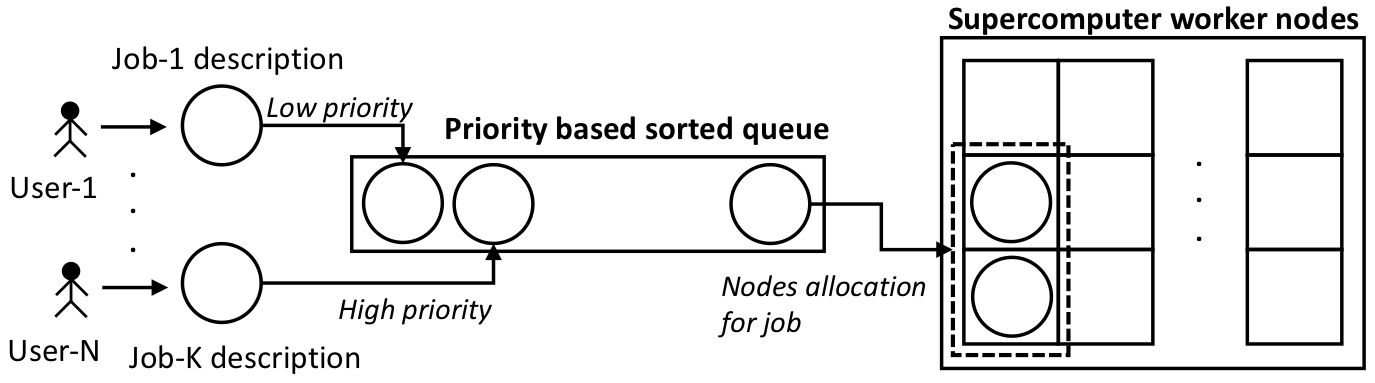
\includegraphics[width=0.45\textwidth]{pics/job-processing-general-scheme.png}
    \caption{General scheme of jobs processing at supercomputers}
    \label{fig-job-processing-general-scheme} 
\end{figure}

It is almost impossible to check through all possible combinations of job
size and requested wall time, since job size can vary from 1 core in 1 node
to the maximum allowable value (e.g., it is more than 18 thousands nodes in
the Titan supercomputer, more details are in Section~\ref{sec-experiments-1-1}),
while wall time can vary from several minutes to several days.
Therefore, we propose to group each parameter's range into small categories,
where jobs from each category can be assumed having similar basic
characteristics, such as, for example, utilization per a single job.

In order to determine a probability of achieving a certain utilization in a
defined time interval for a specified pair $\{num\_nodes, wall\_time\}$, we
have developed a quantitative model.
The model assists in calculation of probability of achieving defined utilization
during the defined time by jobs of certain size with corresponding wall time
(waiting time for a job in the queue is estimated by other parameters).
The model allows to set job's size, wall time and queue waiting time as random
variables with a given expectation and variance.

To determine parameters of a random variable that specifies queue waiting
time for a job of a certain size with corresponding wall time, one can use:
\begin{itemize}
    \item recorded (historical) data;
    \item simulated (synthetic) data.
\end{itemize}

By evaluating recorded (historical) data, it is possible to filter out jobs
with similar characteristics and estimate for them queue waiting time.
The disadvantage of using only recorded (historical) data is that we cannot take
into account changes in system's workload from new jobs, that we will launch
on it.
To take into account such changes, as well as to verify calculations of the
quantitative model, it is possible to use simulated (synthetic) data from a
simulator of the supercomputer load.
This modeling tool was developed in order to meet the analysis requirements.

Figure~\ref{fig-analysis-workflow} illustrates the scheme of the designed
approach, with the following workflow:
i) a user sets the strategy launching schemes;
ii) similar jobs are selected from the log for the given schemes;
iii) for selected jobs, the main characteristics are defined: job size, queue
waiting time, wall time;
iv) if necessary, these characteristics are refined using the simulator;
v) the parameter space is divided into categories and for each category we
calculate probability of achieving the specified utilization using the
quantitative model;
vi) if necessary, utilization calculated for the quantitative model is verified
using the simulator.

\begin{figure}
    \centering
    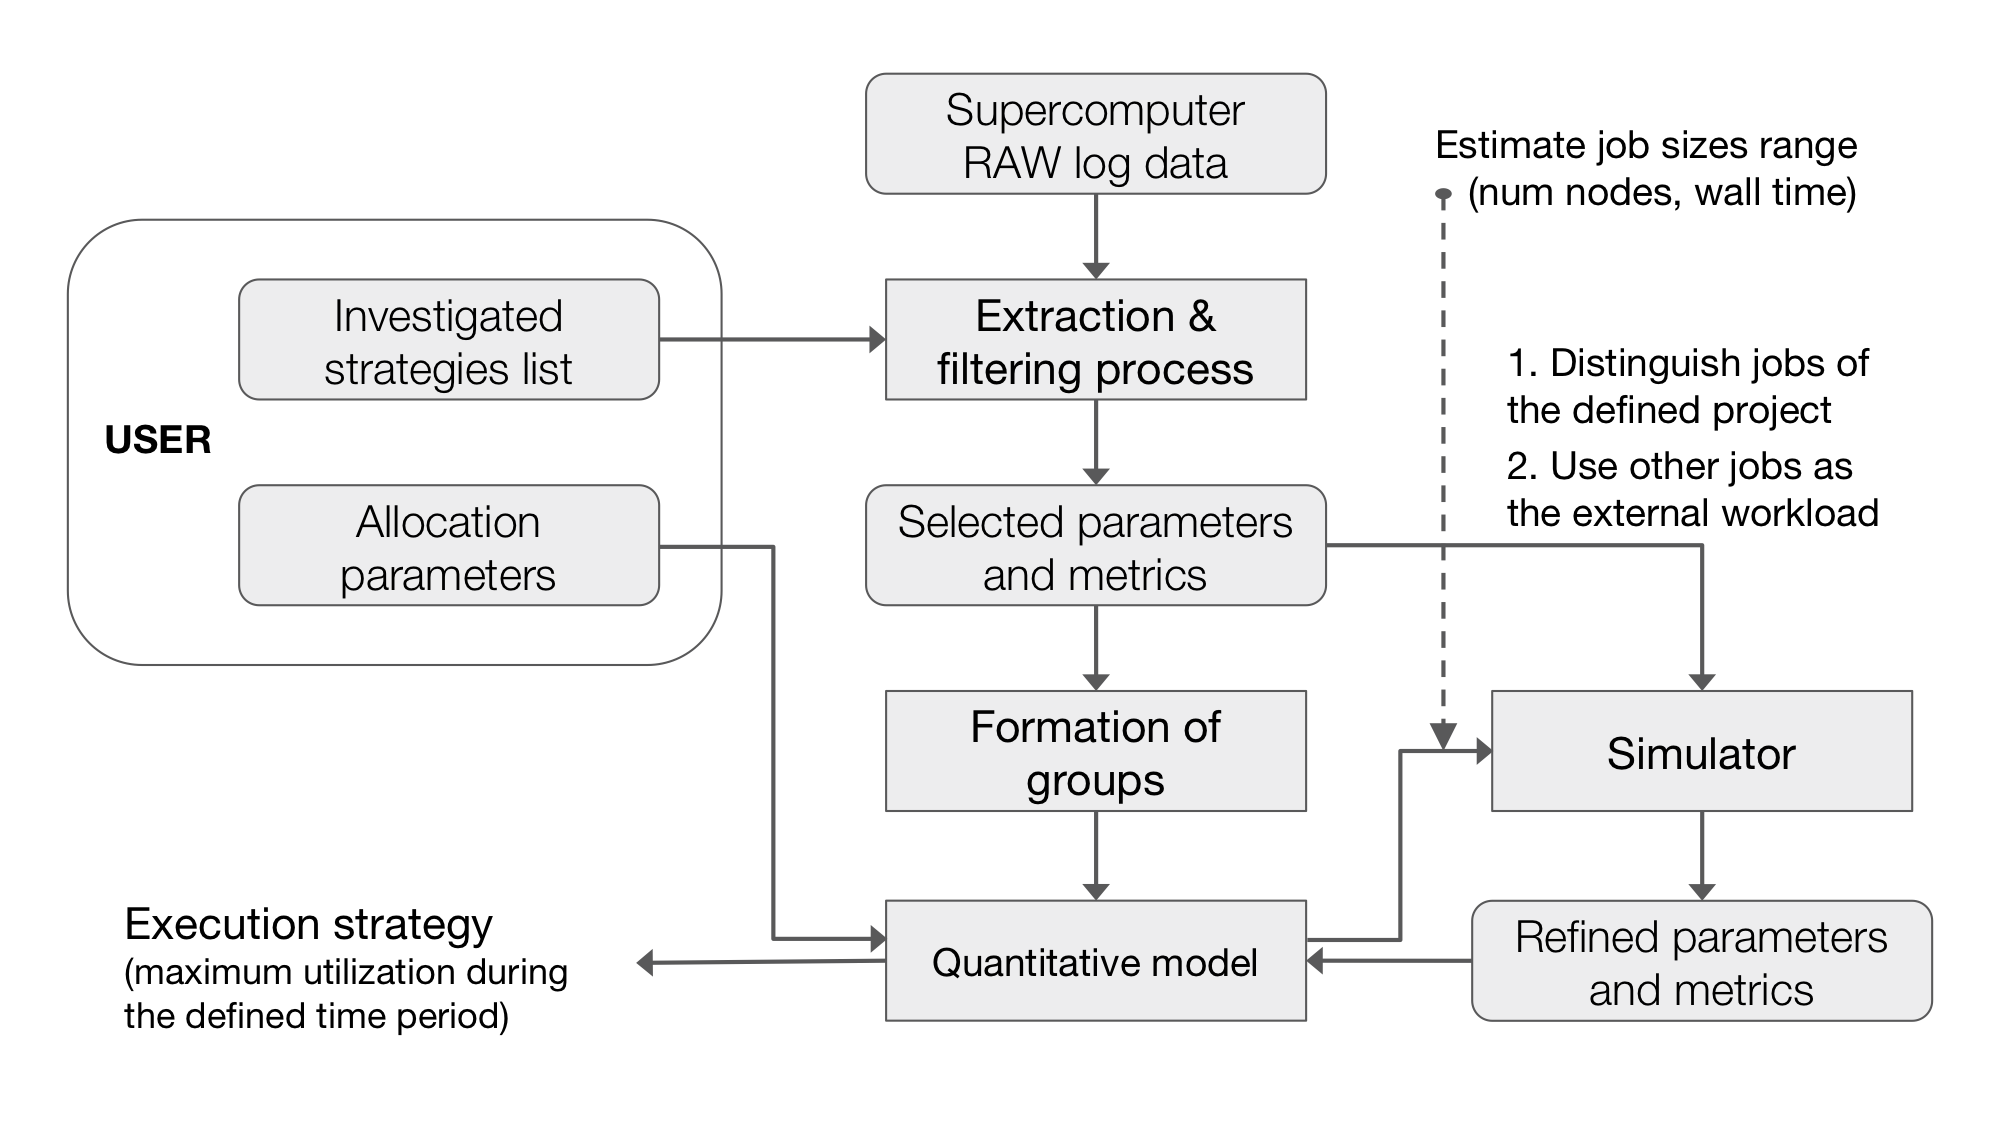
\includegraphics[width=0.48\textwidth]{pics/analysis-workflow.png}
    \caption{Workflow of the analysis process}
    \label{fig-analysis-workflow} 
\end{figure}


\subsection{Modeling tools}
\label{sec-strategy-2}
Designed modeling tools mentioned earlier include the quantitative model for
estimation of the probability of resources utilization with chosen execution
strategy and the simulator that provides a simulation of jobs being executed at
the defined resources (i.e., simulation of workflow's execution), where
resources availability is described by predefined workload based on either
historical log data or synthetic data (simulation of resources utilization for
defined set of jobs with chosen execution strategy).

The simulator provides resulting data (one run of a simulation) for plotting a
distribution of utilization over the simulation time according to the defined
resources workload and the execution strategy for observed jobs.
But this plot might be varying since the process of utilization depends on
random variables.
Thus, many simulations are needed to move from one random result to a
distribution of probabilities, but these are time expensive processes.
On the other hand, the quantitative model gives theoretical calculations on a
distribution of probabilities with defined resources workload and chosen
execution strategy, but it doesn't consider the effect of the applied strategy
on the resources workload.
As the result we have that the simulator provides parameters describing the
state of resources (e.g., workload considering the load from observed jobs with
the defined strategy) and job related characteristics (e.g., a probability of
a single job resource utilization) to the quantitative model to get the
probability estimation of the resources utilization.

\subsubsection{Quantitative Model}
\label{sec-strategy-2-1}

The quantitative model allows to calculate a probability of achieving
required utilization of allocated resources in a given time by defining
specific parameters for jobs processing.
Some of these parameters are set by the user (e.g., the number of requested
nodes and wall time), while other parameters are determined by a particular
workload of a supercomputer and actions (i.e., activity) of other users (e.g.,
the waiting time of the job in the supercomputer's queue before it runs on
compute nodes).
The basic version of the model assumes that jobs, which utilization is under the
estimation, are launched sequentially: every next job arrives to the
supercomputer queue only after the previous job has been started to run on
compute nodes.

Equation that describes the quantitative model (its derivation process is
presented in the Appendix~\ref{appendix-model-derivation}):
\begin{equation}
    \label{eq-quantitative-model}
    \begin{multlined}
    P(U > U_0) = \sum\limits_{n=100}^{\infty} 
                 \bigg[
                 \int_{U_0}^{\infty}f(x, n\mu_{U}, n\sigma_{U}^2)dx \
                 \times \\
                 \bigg( \int_{-\infty}^{T_0}f(x, n\mu, n\sigma^2)dx \  - \\
                 \int_{-\infty}^{T_0}f(x, (n+1)\mu, (n+1)\sigma^2)dx \bigg)
                 \bigg]
    \end{multlined}
\end{equation}

The outcome of the Equation~\ref{eq-quantitative-model} is the probability
that the utilization of resources, which is achieved by a sequential set of
processed jobs using capabilities of the supercomputer during the time
interval $T_0$, is greater than the predefined value $U_0$. It implies that:
\begin{itemize}
    \item Utilization of every single job is described by a random variable
    with the expected value $\mu_{U}$ and the variance $\sigma_{U}^2$;
    \item The time interval between launches of sequential jobs is described
    by a random variable with the expected value $\mu$ and the
    variance $\sigma^2$.
\end{itemize}

\subsubsection{Simulator}
\label{sec-strategy-2-2}

Another modeling tool is the simulator which is aimed to simulate the workload
on a supercomputer and to produce job traces for a given workload, as well,
it is used for the quantitative model validation and adjustment.
There are two modes to run the simulator:
i) set operational parameters, such as job generation rate and job execution
rate, to produce synthetic data only;
ii) use historical data for key parameters of a job, such as timestamp of job
arrival to the queue and job execution time, to produce simulated data of
real job processing life-cycle.
(Detailed description of the simulator is presented in the
Appendix~\ref{appendix-simulator-description}.)


%\subsection{Quantitative model of utilization of allocation time}
%\label{sec-strategy-2}
%The developed model allows to calculate the probability of achieving the required utilization of allocated resources in a given time by defining specific parameters for jobs processing. Some of these parameters are set by the user (e.g., the number of requested nodes and walltime), while other parameters are determined by the workload of the supercomputer and the actions (i.e., activity) of other users (e.g., the waiting time of the job in the supercomputer's queue before it runs on computing nodes).

The base version of the model assumes that jobs, which utilization is under the estimation, are launched sequentially: every next job arrives to the supercomputer queue only after the previous job has been started to run on computing nodes. Also, the model can be adapted to other schemes of jobs launching. For example, if jobs are launched sequentially according to the scheme that ``the every next job enters the queue only after the previous job left it'', then the basic model can be used with ``the virtual waiting time of the job'', which equals to the sum of their real waiting time and their real execution time. If the launching scheme assumes several input streams, e.g., 2-3 streams, then the basic model with one stream can be used, but the defined time for calculated utilization will be reduced by 2-3 times respectively. A formal description of the input and output data for the basic model is presented below.

\textit{Given assumptions}:
\begin{itemize}
    \item Jobs $J$ of project $Pr$;
    \item Jobs $J$ require $N$ nodes, where $N$ is a random variable with expected value $\mu_{N}$ and variance $\sigma_{N}^2$;
    \item Jobs $J$ require walltime $E$, where $E$ is a random variable with expected value $\mu_{E}$ and variance $\sigma_{E}^2$;
    \item Execution times of jobs $J$ equal to their walltime values;
    \item Duration of waiting time in the queue for jobs $J$ is described by a random variable $Q$ with expected value $\mu$ and variance $\sigma^2$;
    \item Jobs $J$ come into the supercomputer queue sequentially: the next job is allocated to the queue after the previous one has left the queue to computing nodes.
\end{itemize}

\textit{Values to find}:
$P(U > U_0)$ - the probability that utilization $U$ during the time interval $T_0$ will exceed the predefined value $U_0$, where $T_0$ is big.

The derivation process is presented in the appendices (Appendix~\ref{appendix-model-derivation}), and here is the final equation that describes the quantitative model:
\begin{equation}
    \label{eq-quantitative-model}
    \begin{multlined}
    P(U > U_0) = \sum\limits_{n=100}^{\infty} 
                 \bigg[ \int_{U_0}^{\infty}f(x, n\mu_{U}, n\sigma_{U}^2)dx \  \times \\
                 \bigg( \int_{-\infty}^{T_0}f(x, n\mu, n\sigma^2)dx \  - \\
                 \int_{-\infty}^{T_0}f(x, (n+1)\mu, (n+1)\sigma^2)dx \bigg) \bigg]
    \end{multlined}
\end{equation}

The outcome of the Equation~\ref{eq-quantitative-model} is the probability that the utilization of resources, which is achieved by a sequential set of processed jobs using capabilities of the supercomputer during the time interval $T_0$, is greater than the predefined value $U_0$. It implies that:
\begin{itemize}
	\item Utilization of every single job is described by a random variable with the expected value $\mu_{U}$ and the variance $\sigma_{U}^2$;
	\item The time interval between launches of sequential jobs is described by a random variable with the expected value $\mu$ and the variance $\sigma^2$.
\end{itemize}


%\subsection{Simulator}
%\label{sec-strategy-3}
%This designed analysis tool is aimed to simulate the workload on a supercomputer and to produce job traces for a given workload, as well, it is used for the quantitative model validation and adjustment. There are two modes to run the simulator: i) set operational parameters, such as job generation rate and job execution rate, to produce synthetic data only; ii) use historical data for key parameters of the job, such as timestamp of job arrival to the queue and job execution time, to produce simulated data of real job processing life-cycle.

The simulator is based on Queueing Theory~\cite{ref-queueing-theory} and according to the Kendall's Notation~\cite{ref-kendall} for queues, usually referred as A/B/C/D/E, it is characterized as following:
\begin{itemize}
    \item A - \textit{arrival process} is represented by streams that are responsible for job generation and is described either by a Poisson process or by a deterministic model;
    \item B - \textit{service/server process} is represented by a set of nodes that simulate job execution process and is described either by a Poisson process or by a deterministic model as well;
    \item C - \textit{number of servers} that corresponds to the number of computing nodes (in terms of the Titan supercomputer);
    \item D - \textit{capacity of the queue or system overall}, which is ``on'', if the queue limit is set (either per stream or for the total number of jobs in the queue) and queue buffer is not used, otherwise the capacity is unlimited;
    \item E - \textit{queueing discipline} is provided in two options: FIFO or Priority.
\end{itemize}

Some of the parameters are set as requirements and restrictions applied to a specific supercomputer and its policy, e.g., the total number of computing nodes that are available for computing jobs, the limit of the number of jobs in the queue per user/group, etc.

\subsubsection{Simulator description} \label{sec-strategy-3-1}

Implementation of the simulator (Queueing System Simulator) \cite{ref-qss} was done by using Python\footnote{High-level programming language Python, \url{https://docs.python.org/2.7/} [accessed on 2019-04-15]}, and the following key classes and generators were designed (to emulate internal supercomputer processes): 
\begin{itemize}
    \item \textit{Job} - contains parameters to describe job's processing life-cycle, such as arrival timestamp, start execution timestamp, completion timestamp that is based on walltime / execution time along with the previous parameter, number of required nodes for its execution, stream (i.e., source name), label (i.e., project name), priority and priority group name;
    \item \textit{Stream} - generates jobs with the predefined parameters as an input for the simulator;
    \item \textit{Queue Manager} - emulates buffer ahead of the queue, the queue itself, and manages jobs while waiting for their execution, it lets to define the queue discipline such as FIFO and Priority, and set the limits per input job stream;
    \item \textit{Schedule Manager} - emulates a backfill mode - gets information about job sizes, assigns corresponding nodes for execution, gives a schedule when each job starts to be executed;
    \item \textit{QSS} - the core class that manages and tracks job's processing life-cycle.
\end{itemize}

\subsubsection{State model} \label{sec-strategy-3-2}

Job life-cycle (in terms of the simulator, Figure~\ref{fig-simulator-scheme}) includes the following states: Generated - Holding (i.e., Titan notation: blocked) [buffer] - Pending (i.e., Titan notation: eligible-to-run) [queue] - Starting - Executing - Finished. Some of the states might be skipped if certain components are turned off (e.g., if the queue buffer is not used then there is no state ``holding'') or if there is some initial restriction (e.g., state ``starting'' is neglected, since the assumption that job execution starts right after it leaves the queue).

\begin{figure}
    \centering
    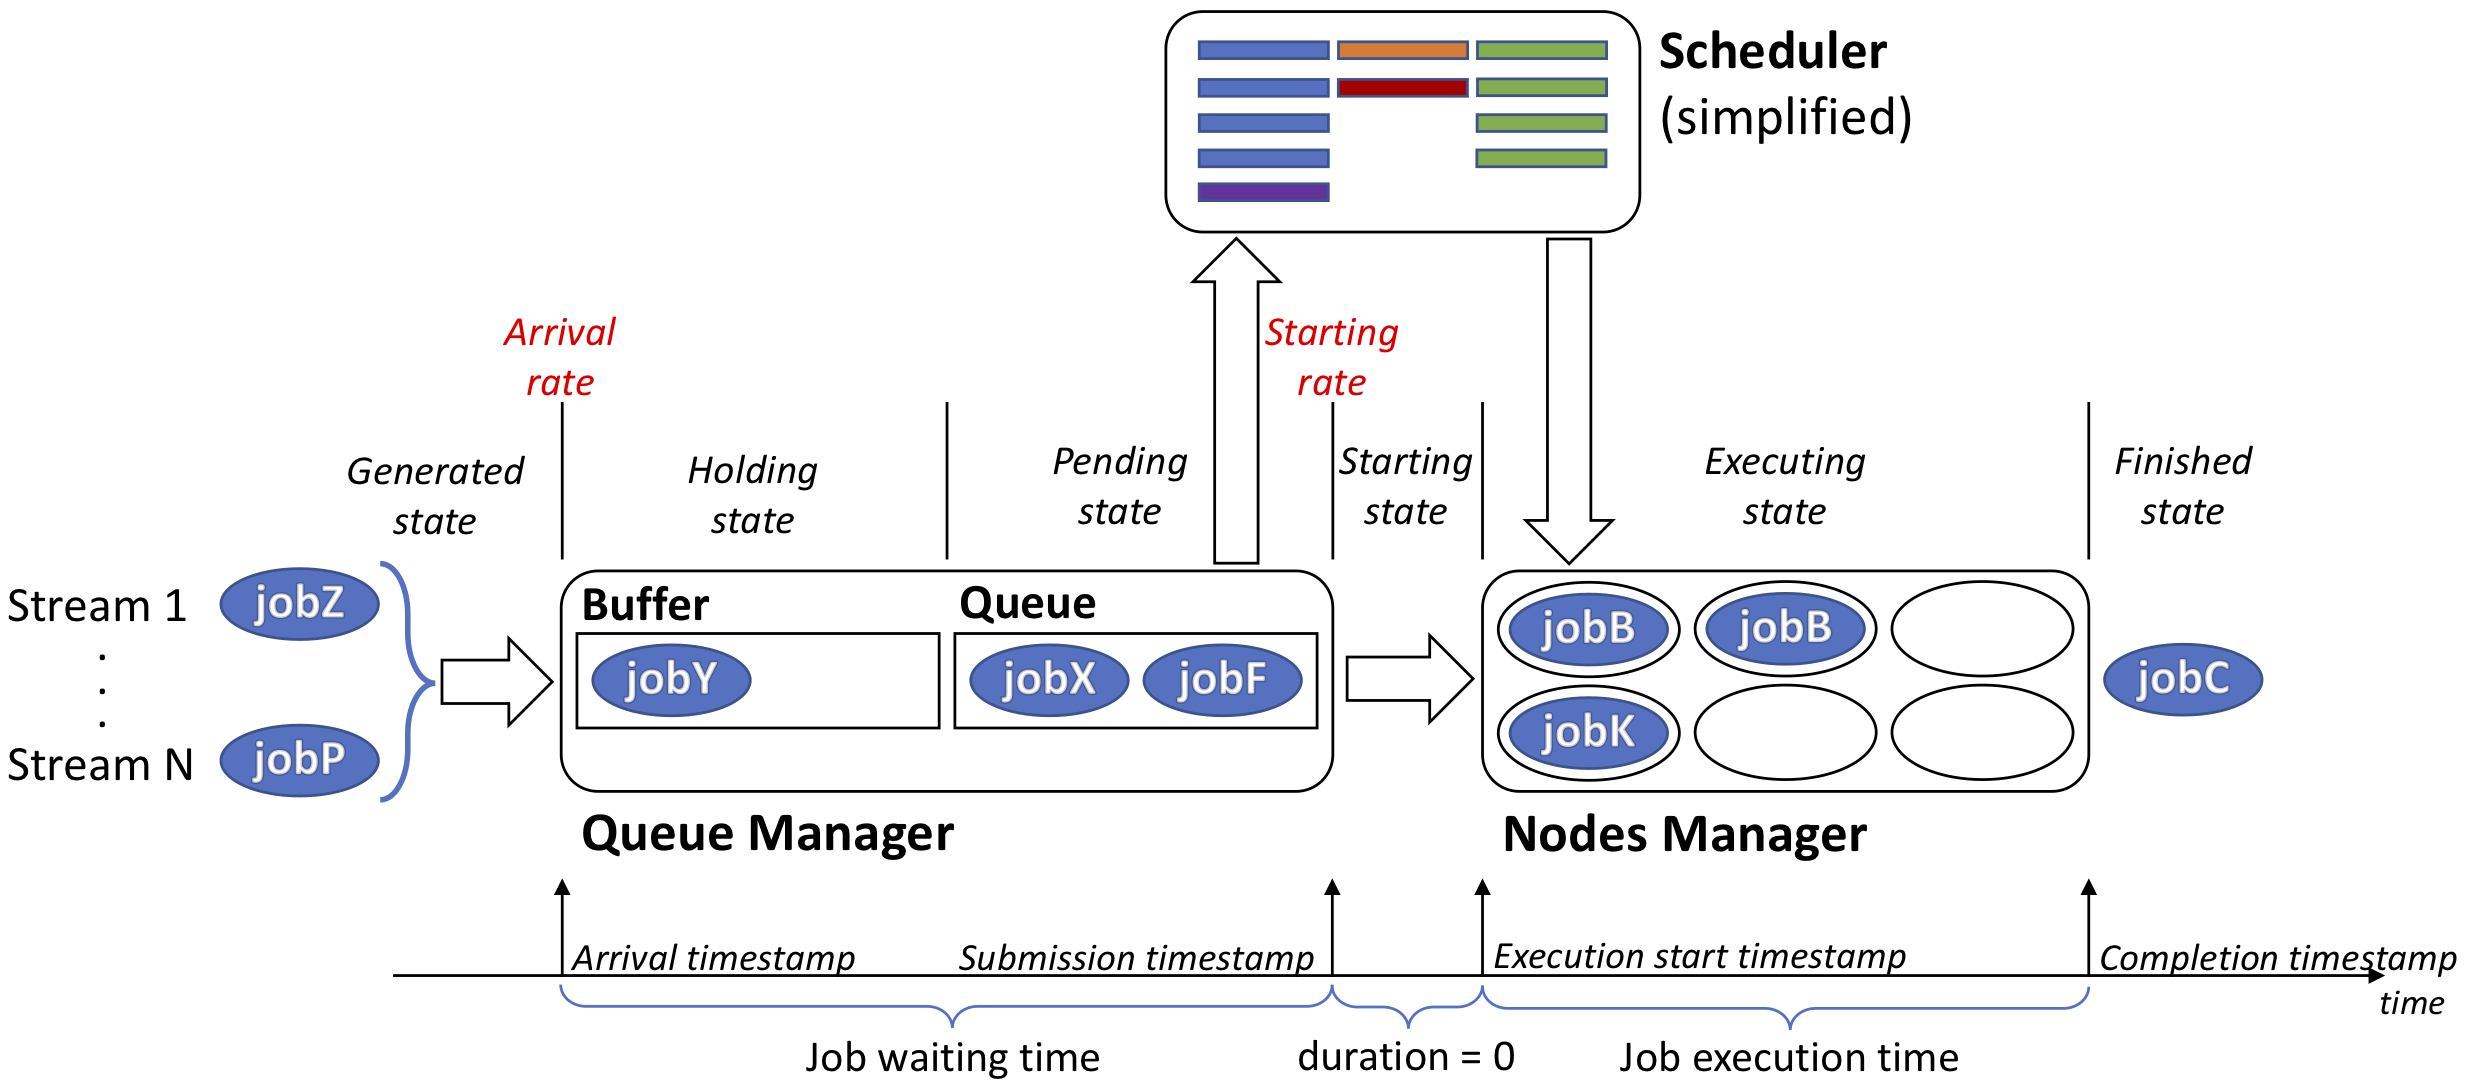
\includegraphics[width=0.48\textwidth]{pics/simulator-scheme.png}
    \caption{Job state transitions at the simulator}
    \label{fig-simulator-scheme} 
\end{figure}


\subsection{Testing and validation}
\label{sec-strategy-3}
\subsubsection{Model validation using utilization estimation} \label{sec-strategy-4-1}

The validation of the designed quantitative model was conducted based on a simplified model for which utilization is computed using theoretical calculations. The following conditions have been applied:
\begin{itemize}
	\item Starting rate of jobs is defined as a random variable with distribution denoted as SRD;
	\item Execution time of jobs is defined as a random variable with distribution denoted as ETD;
	\item Number of nodes used (requested) by examined jobs is defined as a random variable with distribution denoted as NND.
\end{itemize}

With this model it is possible to estimate the expected utilization achieved in a given long period of time. The expected utilization $U(t)$ depends on particular values of the random values in it, therefore it is mutable. But for big numbers of the time $t$ it is possible to take advantage of the law of large numbers (LLN). In this case, it can be argued that the value of $U(t)$ will tend to the same value, regardless of particular values of the random variables within it.

The theoretically calculated utilization for large values of $t$ can be estimated by the following equation:
\begin{equation}
	\label{eq-theoretical-utilization}
	U(t) \approx t \times E(SRD) \times E(ETD) \times E(NND)
\end{equation}
where $E(x)$ is the expected value (mathematical expectation) of a random variable. The next step was to compare the outcome of Equation~\ref{eq-quantitative-model} (model) and Equation~\ref{eq-theoretical-utilization} (theoretical estimation). Thereby, the expected value was calculated approximately, while going from the distribution function of a random variable to the utilization derivation.

Parameters of the experiment:
\begin{itemize}
	\item Starting rate is a random variable with the Poisson distribution, the event rate (i.e., rate parameter and considered as an expected value) $\lambda = 100$;
	\item Execution time is a random variable with the Normal distribution, mean of the distribution $\mu = 4$;
	\item Number of nodes used by a single job is a random variable with the Poisson distribution, $\lambda = 8$;
	\item Examined time interval is half a year $\approx4320\ hours$.
\end{itemize}

Results of the experiment: the utilization calculated using Equation~\ref{eq-quantitative-model} is equal to $13,822,864$, while the utilization calculated using Equation~\ref{eq-theoretical-utilization} (theoretical, based on expected values of SRD, ETD, NND only) is equal to $13,824,000$. Thus, the results are very close, and the little difference is due to approximations related to conducted computations.


\subsubsection{Model validation based on mathematical calculations and synthetic data from the simulator} \label{sec-strategy-4-2}

The further analysis of the quantitative model and the simulator is a simplified validation process that demonstrates equal results of both with the same input data.

The following common parameters are chosen: 
\begin{itemize}
    \item the total number of nodes is equal to 1;
    \item expected value ($\mu$) and variance ($\sigma^2$) for random parameters of job's waiting and execution times respectively are equal to 1; 
    \item the total processing time is equal to 5000 time units (hours).
\end{itemize}

Simulation process follows additional specific parameters:
\begin{itemize}
    \item job waiting time is defined according to the Poisson distribution;
    \item job execution time is defined according to the Normal distribution;
    \item job launching scheme: one stream and there is always one job in the queue;
    \item the total number of simulation runs is equal to 100.
\end{itemize}
Figure~\ref{fig-simulation-and-modeling} shows the plot with two lines that represent the probability that a given utilization will be achieved in a given time interval (that is defined by the total processing time): the blue line corresponds to the results obtained using the simulator, while the red line corresponds to calculations with the quantitative model.

\begin{figure}
    \centering
    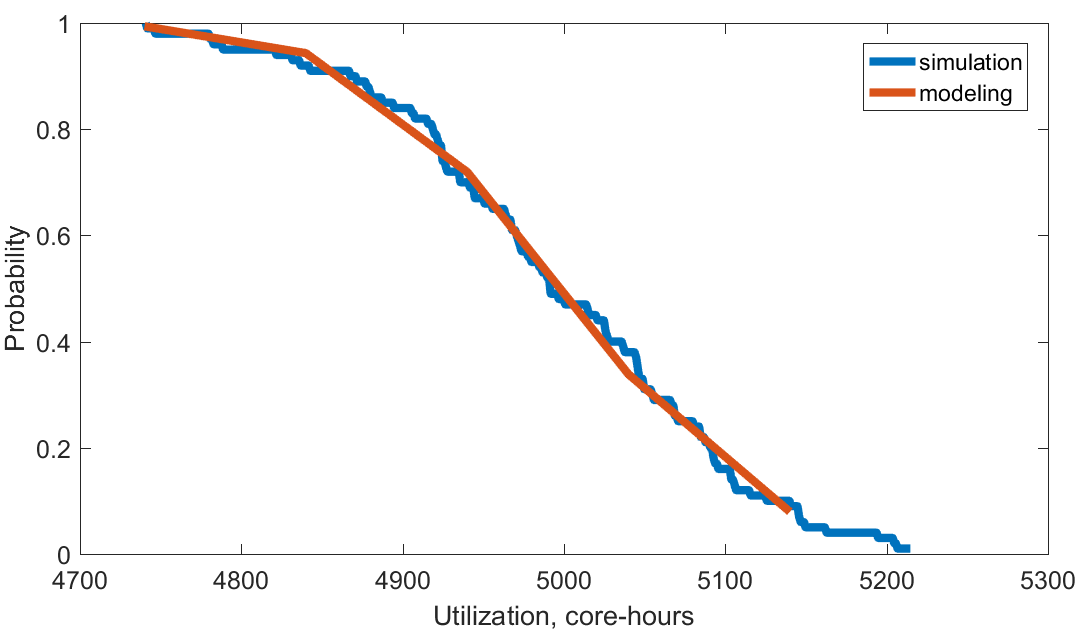
\includegraphics[width=0.48\textwidth]{pics/simulation-and-modeling.png}
    \caption{Probability (axis Y) that utilization will reach the corresponding utilization value (axis X) during the time of 5000 hours}
    \label{fig-simulation-and-modeling} 
\end{figure}



\section{Experiments}
\label{sec-experiments}

\subsection{Background of the study}
\label{sec-experiments-1}
\subsubsection{The Titan supercomputer}
\label{sec-experiments-1-1}

One of the supercomputers that we consider as a use case for modeling allocation utilization is Titan that is located at the Oak Ridge Leadership Computing Facility (OLCF) in the Oak Ridge National Laboratory (USA). Titan\footnote{The Titan supercomputer, \url{https://www.olcf.ornl.gov/olcf-resources/compute-systems/titan/} [accessed on 2019-04-15]} is a hybrid-architecture Cray XK7 system that contains both CPUs (16-core AMD Opteron) and GPUs (NVIDIA Kepler). It features 18,688 compute nodes, a total system memory of 710 TB, and Cray's high-performance Gemini network. Titan's theoretical peak performance exceeding 27 petaFLOPS.

The general overview of jobs processing at the Titan supercomputer is presented by the following plots (Figures~\ref{fig-titan-logs-waiting-time},~\ref{fig-titan-logs-execution-time}) that demonstrate metrics such as waiting and execution times, as well as requested and eventually used nodes per job (Figure~\ref{fig-titan-logs-nodes-count}) during the defined period of time.

Quantitative characteristics of the presented plots are the following:
\begin{itemize}
    \item waiting time (hours): mean=6.21, std=29.77
    \item execution time (hours): mean=0.61, std=1.51
    \item number of nodes per job: mean=135.07, std=712.31
\end{itemize}
These numbers give a general overview of jobs key characteristics while processing at the Titan supercomputer, and which are compared with the results of simulation runs (outcome of the simulator).

\begin{figure}
    \centering
    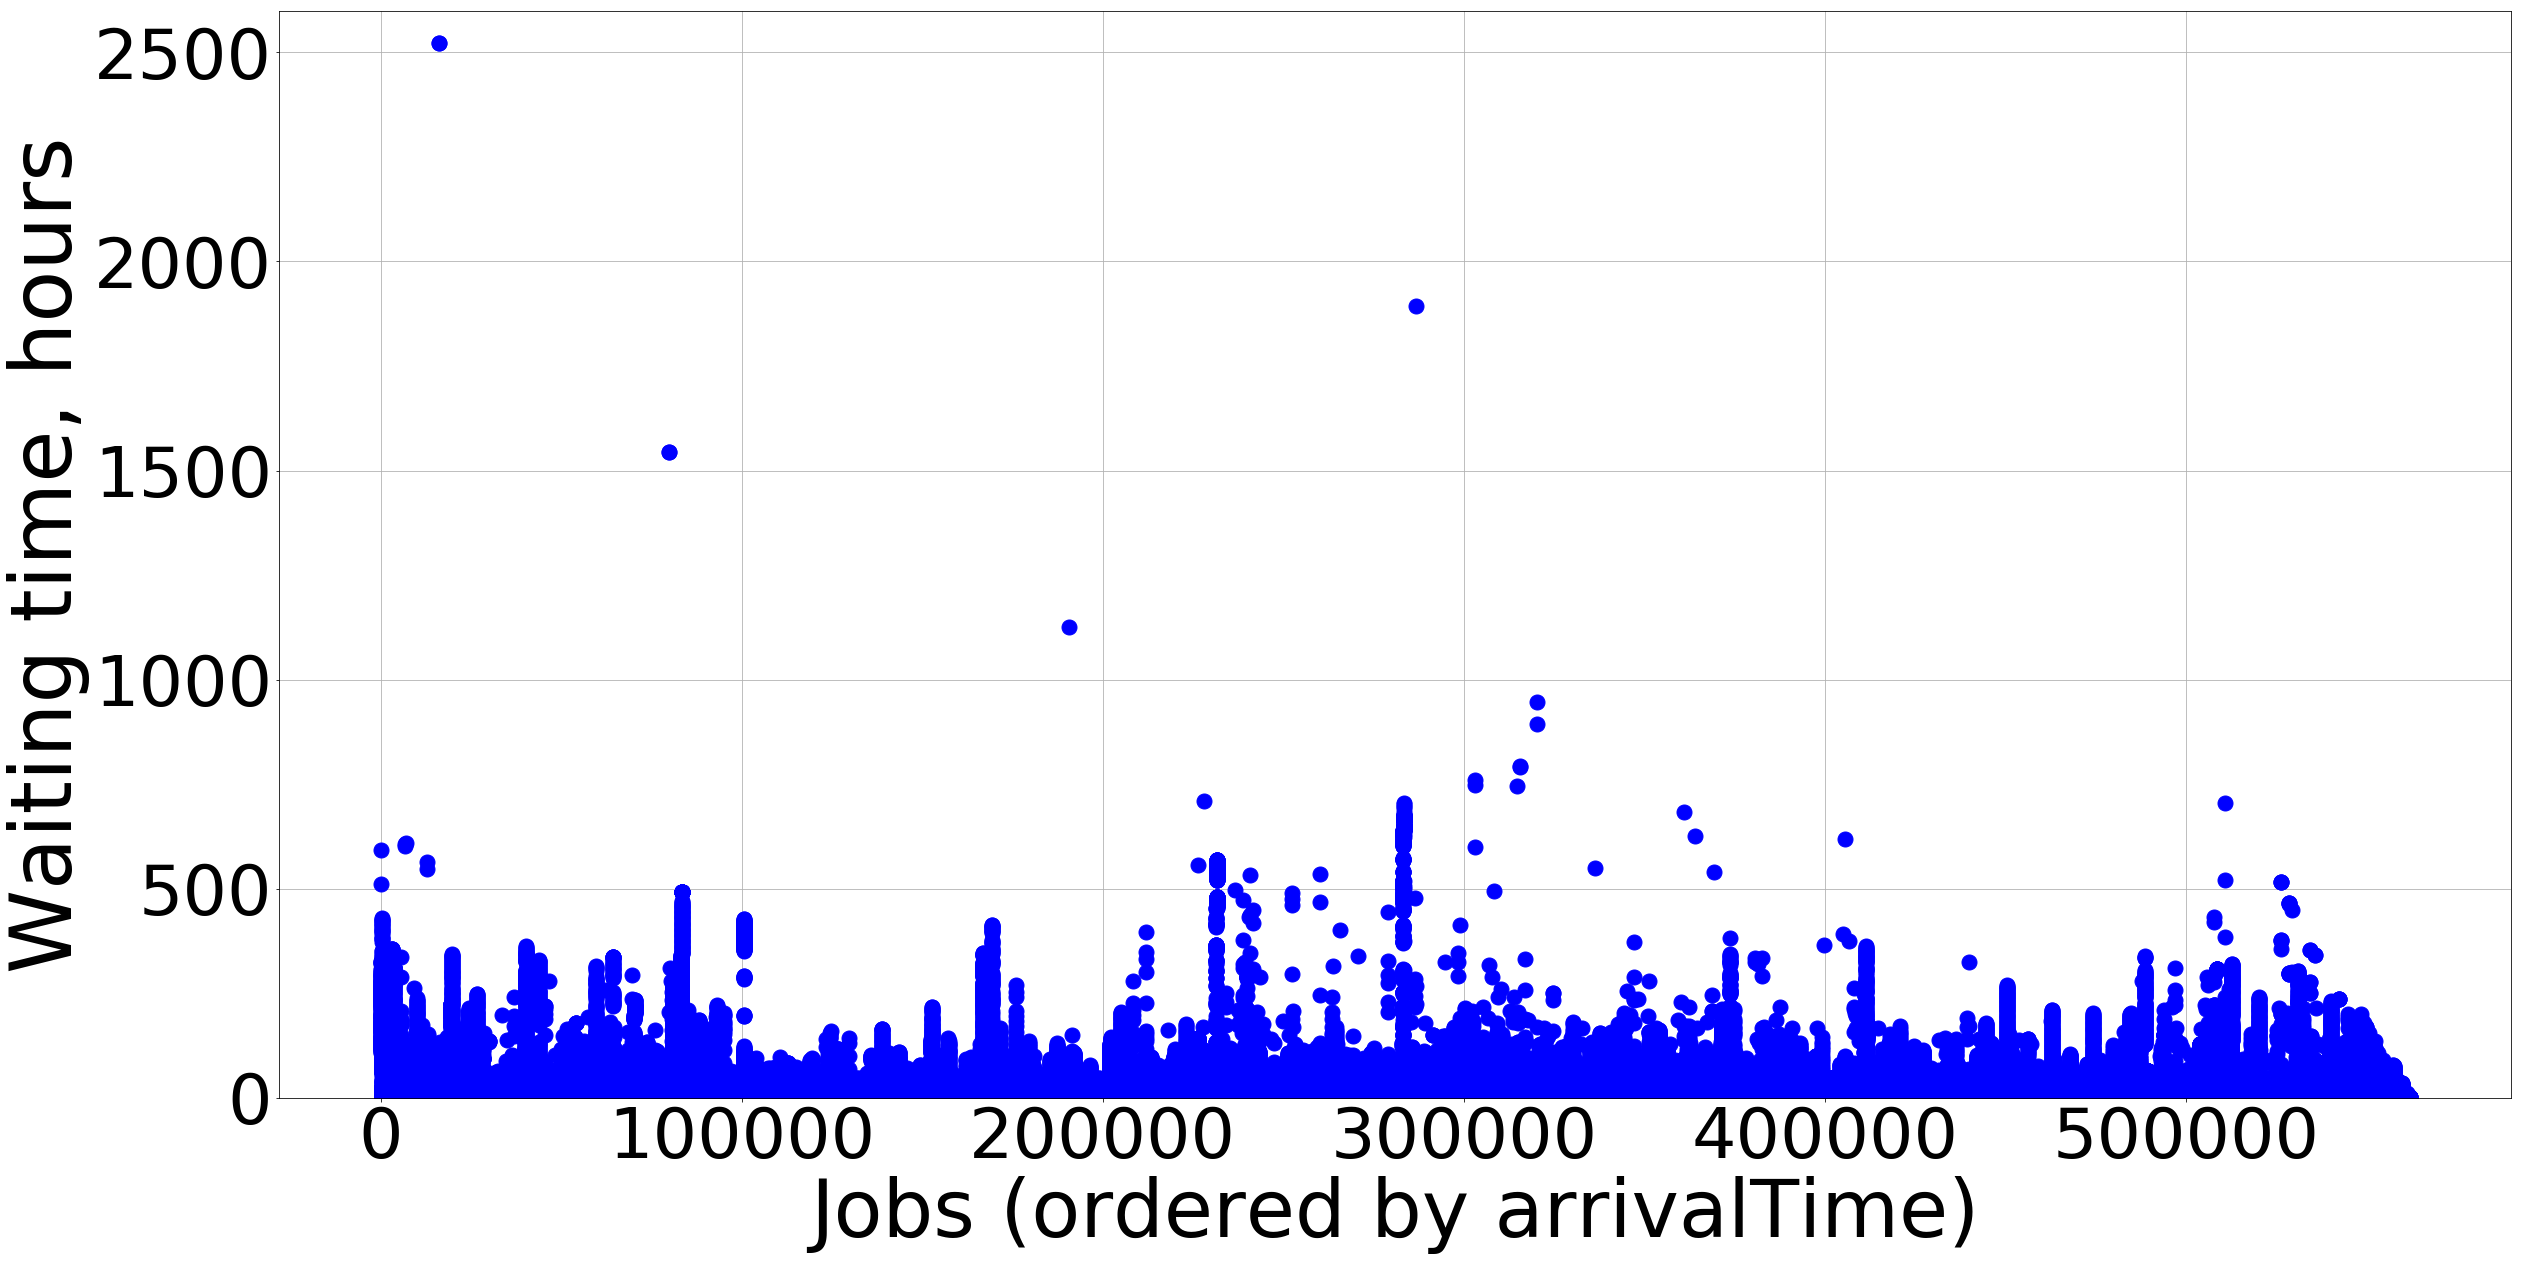
\includegraphics[width=0.45\textwidth]{pics/titan-logs-waiting-time.png}
    \caption{Waiting times for jobs in the queue at the Titan supercomputer (562,079 computing jobs from May 2017 to April 2018)}
    \label{fig-titan-logs-waiting-time} 
\end{figure}

\begin{figure}
    \centering
    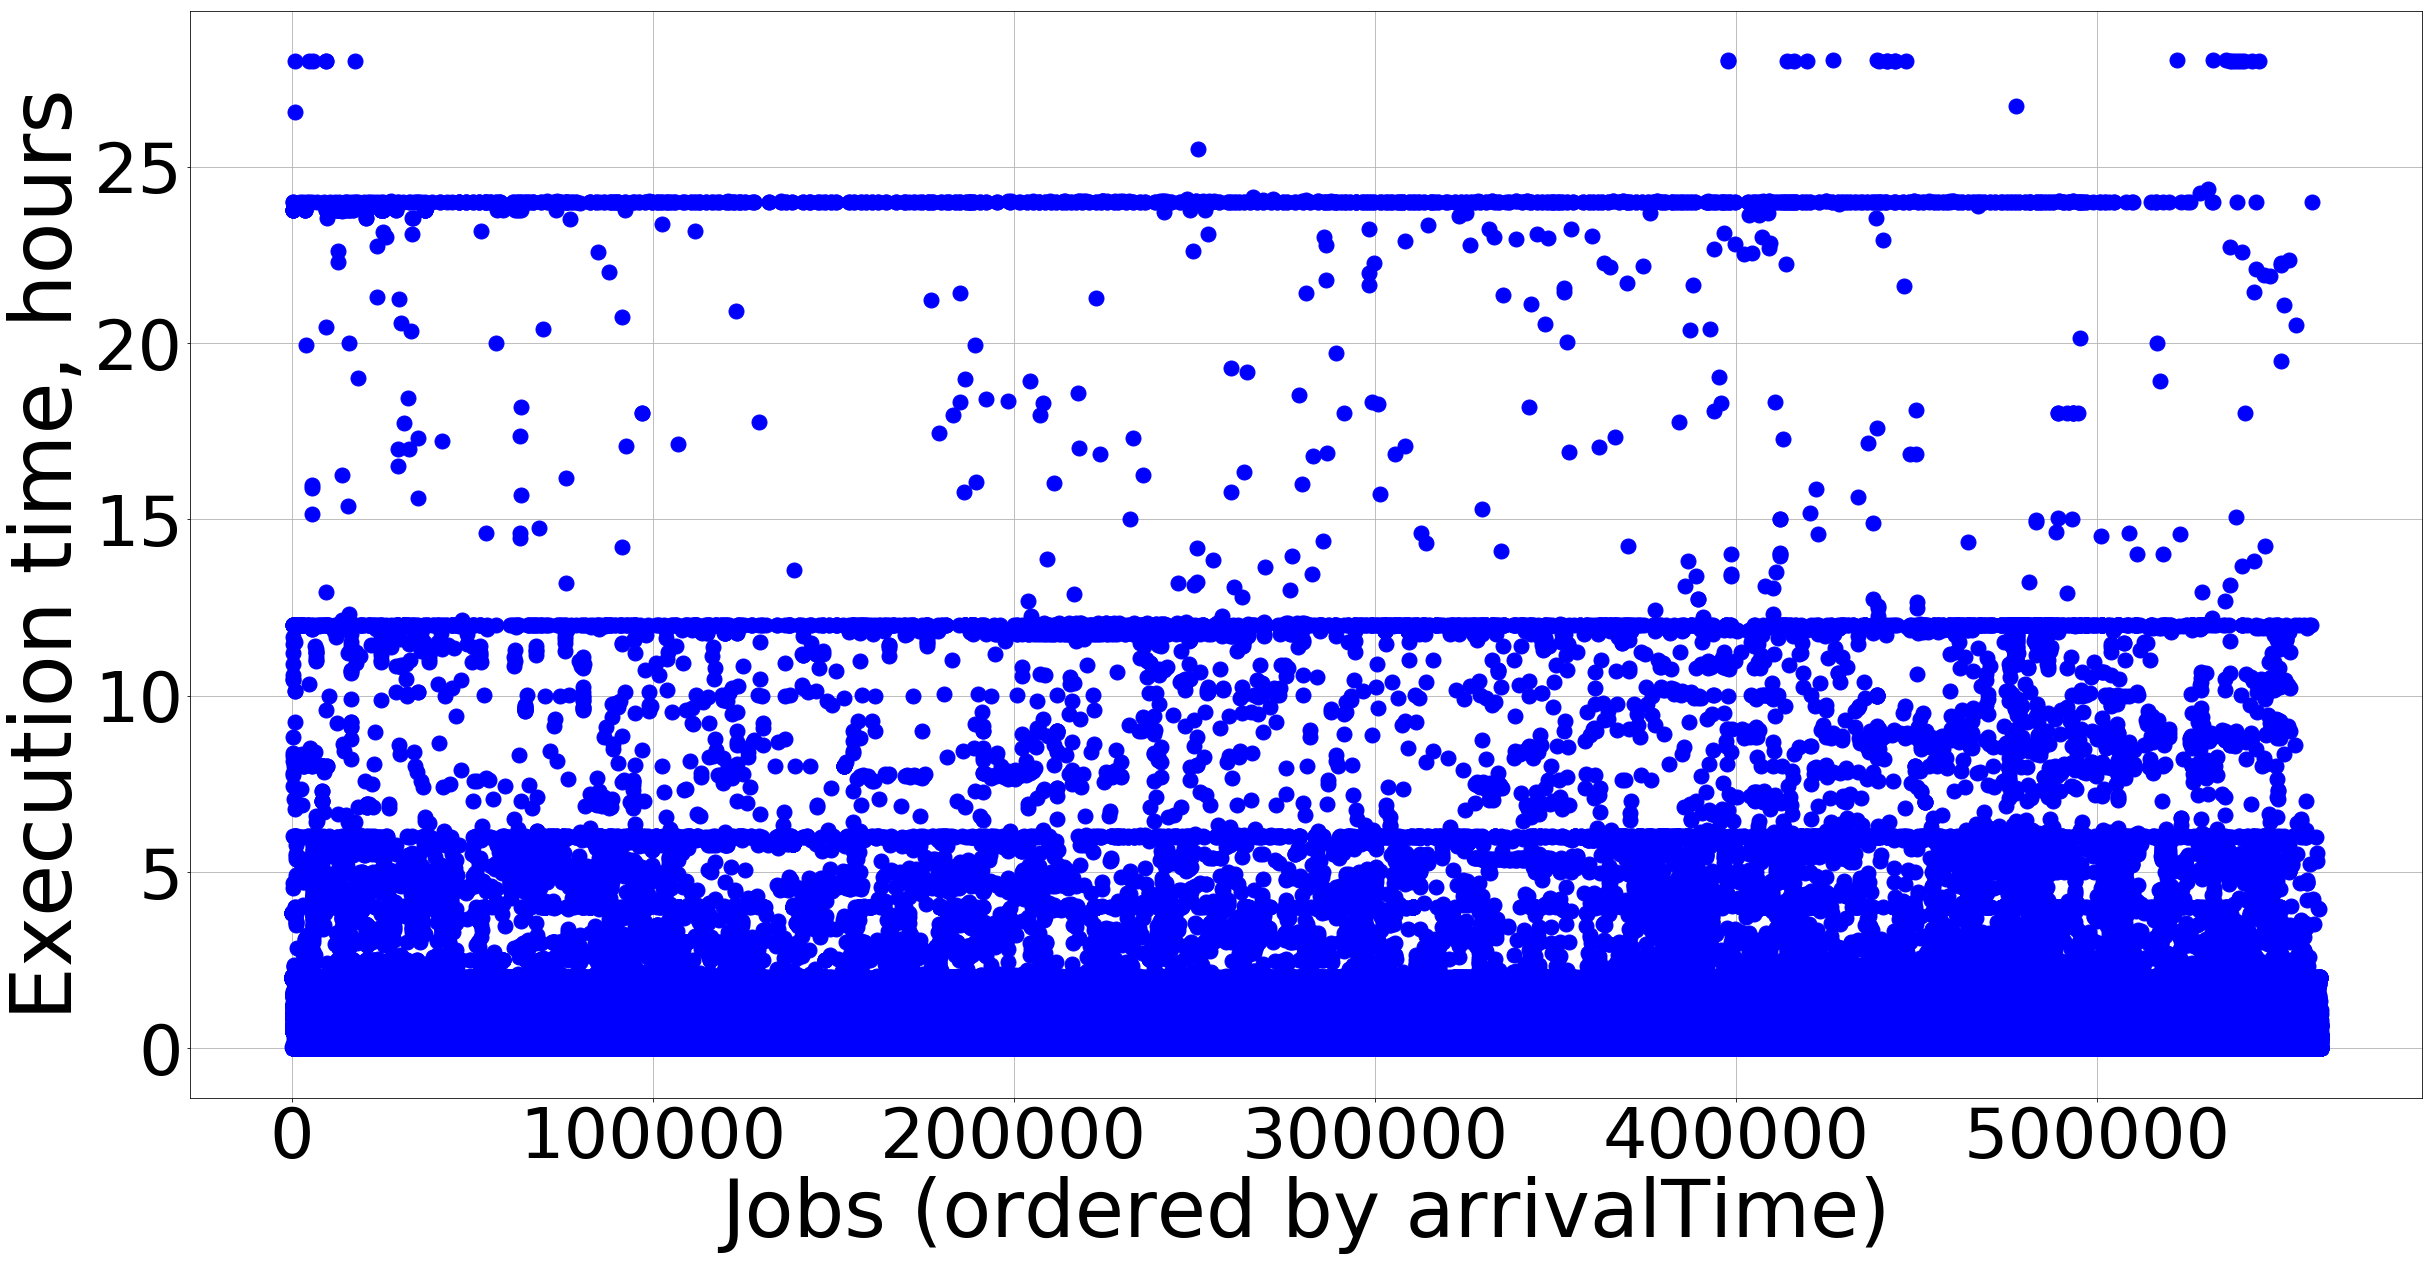
\includegraphics[width=0.45\textwidth]{pics/titan-logs-execution-time.png}
    \caption{Execution times for jobs processing at the Titan supercomputer (562,079 computing jobs from May 2017 to April 2018)}
    \label{fig-titan-logs-execution-time} 
\end{figure}

\begin{figure}
    \centering
    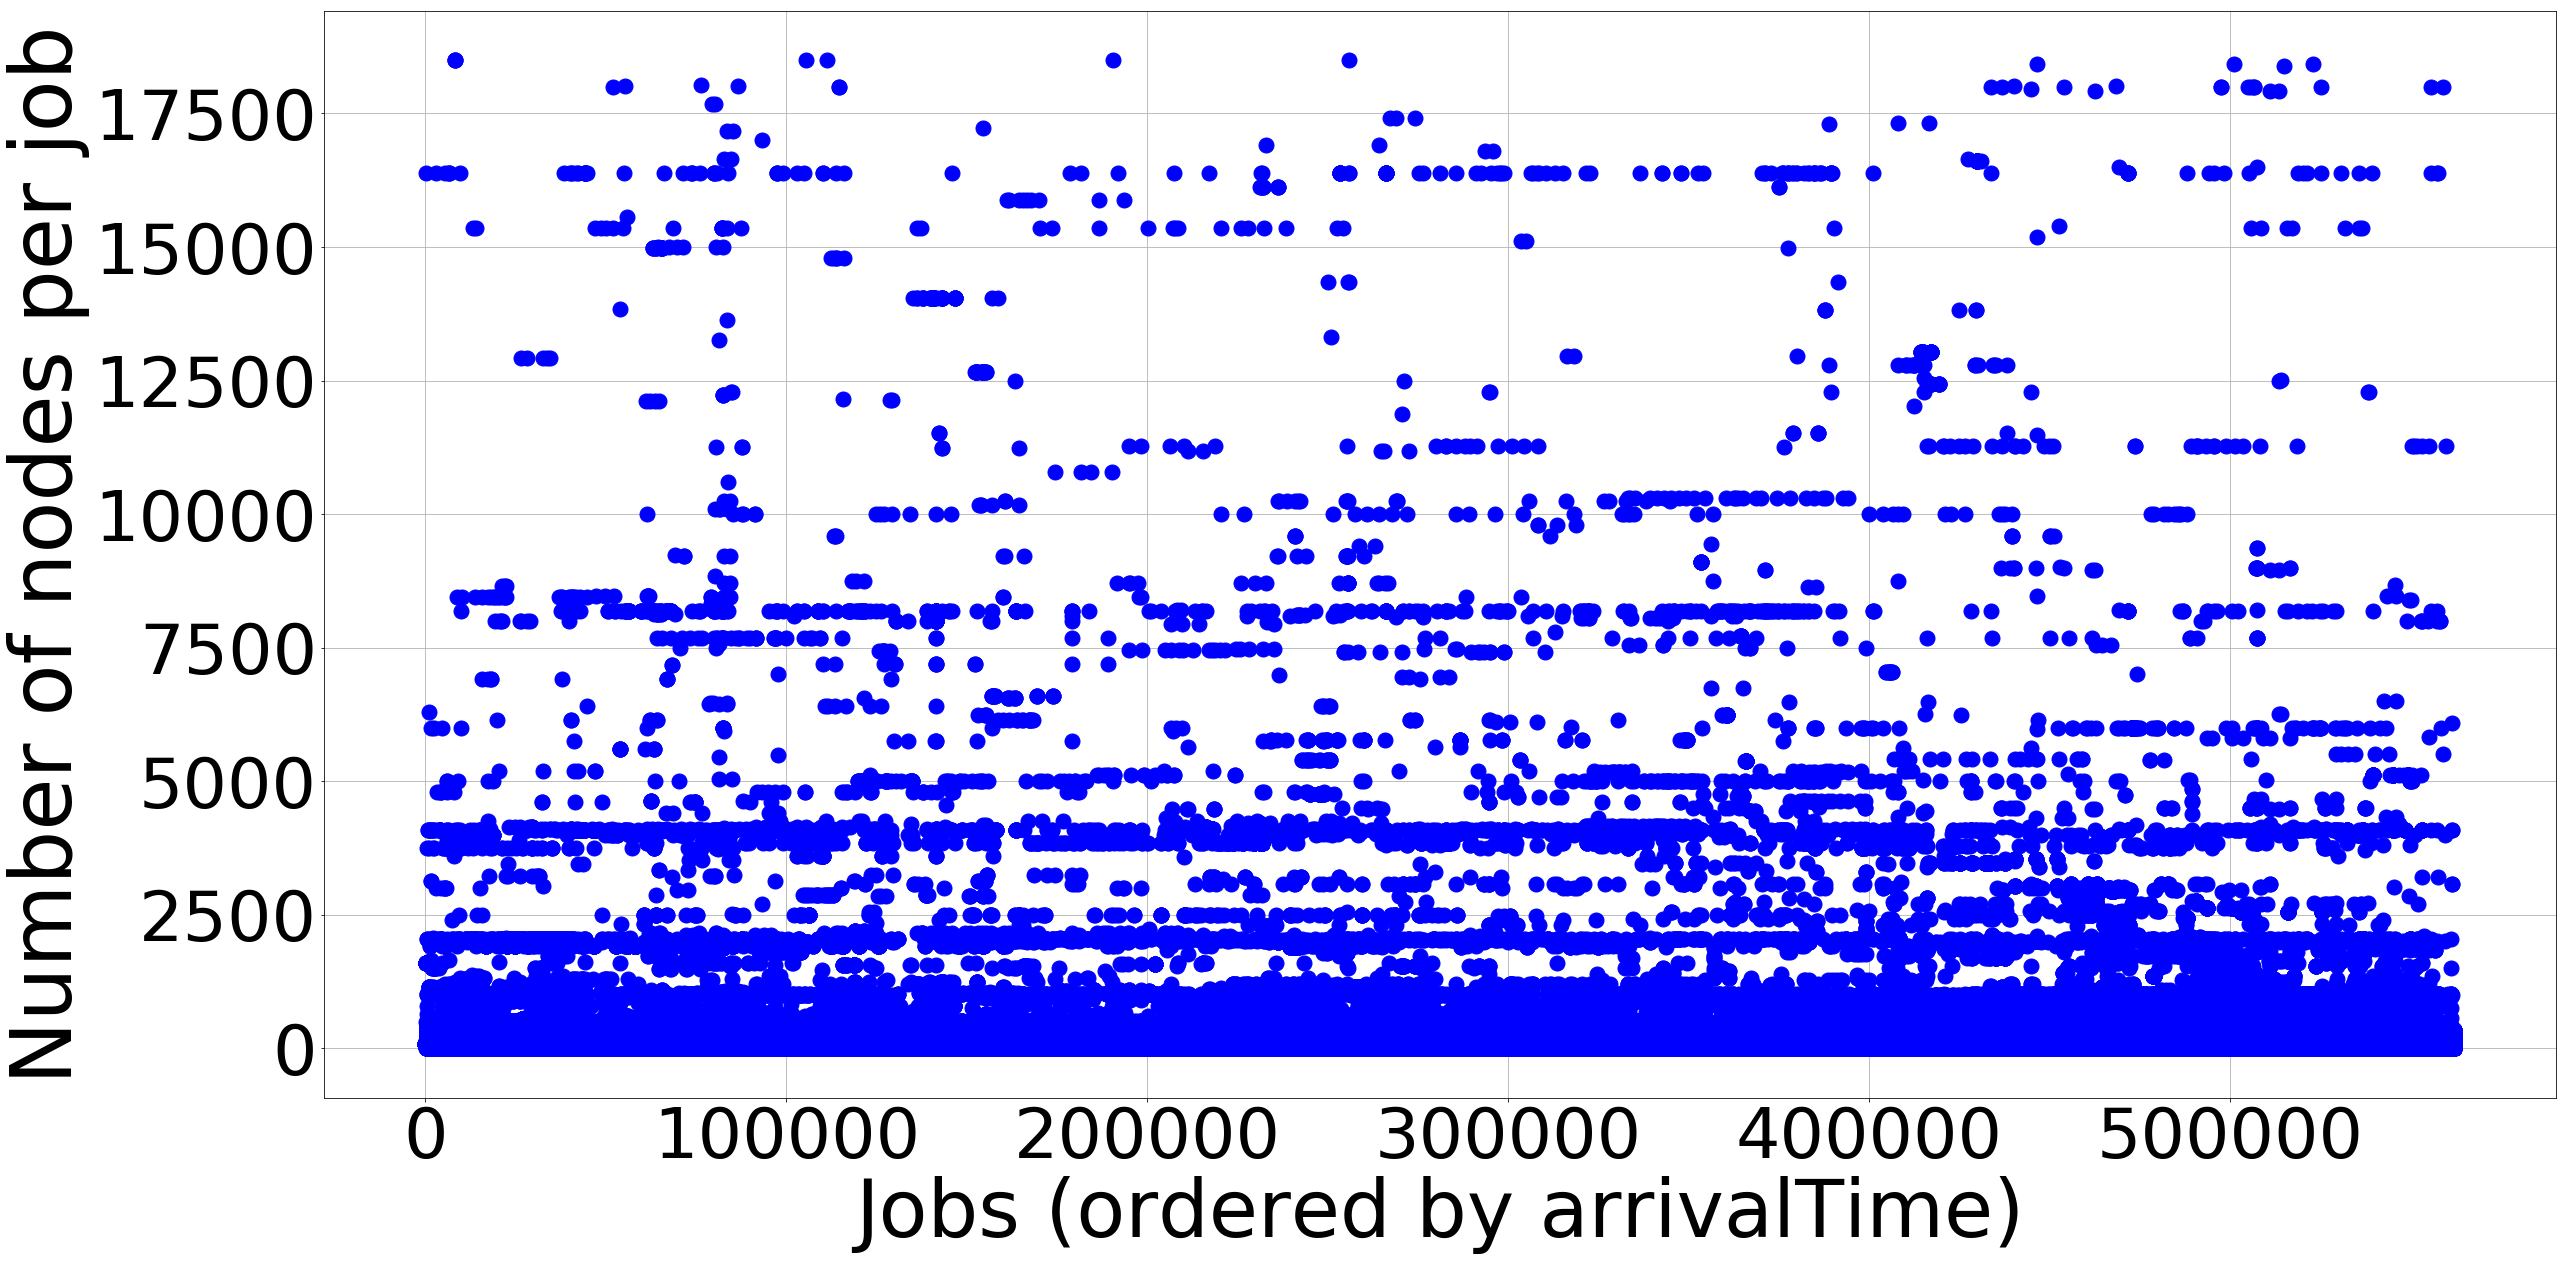
\includegraphics[width=0.45\textwidth]{pics/titan-logs-nodes-count.png}
    \caption{Number of nodes per job at the Titan supercomputer (562,079 computing jobs from May 2017 to April 2018)}
    \label{fig-titan-logs-nodes-count} 
\end{figure}

\subsubsection{Production and Distributed Analysis system PanDA} \label{sec-experiments-1-2}

The PanDA (Production and Distributed Analysis) system is a workload management system (WMS) for job scheduling on the distributed computational infrastructure~\cite{ref-panda}, it federates hundreds of heterogeneous computing resources (including Grid, supercomputers, and public and private computing clouds) into a unique job submission system. It was originally developed for US physicists and adopted as the ATLAS~\cite{ref-atlas} wide WMS in 2008 (in use for all computing applications of the ATLAS experiment at the Large Hadron Collider).

Key features of PanDA are the following: i) pilot-based job execution system with late binding (i.e., there is a lightweight process scheduled on computing nodes that interacts with the core to schedule computing jobs); ii) central job queue; iii) fair-share or policy driven priorities for thousands of users and hundreds of resources; iv) automated brokerage based on CPU and storage resources.

PanDA started to use the Titan supercomputer as one of its resources several years ago under the project of integration with it by enhancing with tools and methods relevant to work on HPC~\cite{ref-titan-prodsys}. Thus, the pilot runs on Titan's data transfer nodes (DTNs) and submits corresponding payloads to the worker nodes. It uses the local job scheduling and management system (Moab) via the SAGA (Simple API for Grid Applications) interface~\cite{ref-saga} for monitoring and management of PanDA jobs running on Titan's worker nodes.

In 2017, under the ALCC\footnote{ALCC: the ASCR (Advanced Scientific Computing Research) Leadership Computing Challenge, \url{https://science.energy.gov/ascr/facilities/accessing-ascr-facilities/alcc/} [accessed on 2019-04-15]} program it was allocated computational resources ($cores \times hours$, i.e., computing hours) at the OLCF supercomputer Titan for ATLAS payload via PanDA.


\subsection{Simulator with Titan log data}
\label{sec-experiments-2}
The following parameters correspond to the Titan supercomputer: 
1) number of nodes is 18,688; 
2) the limit of jobs in the queue per stream is 4; 
3) the queue buffer is on - that corresponds to no dropped jobs.

Obtained Titan log data (for the period from May 2017 to April 2018) were used in the simulator to test it. Certain job parameters were used for deterministic models for arrival and service processes in the simulator, thus Titan log data provided the following jobs characteristics: arrival timestamp (timestamp of queueing), number of requested nodes per job, real execution time. Also, there are restrictions and requirements applied to the queue (according to the Titan Scheduling Policy\footnote{Titan Scheduling Policy, \url{https://www.olcf.ornl.gov/for-users/system-user-guides/titan/titan-user-guide/#titan-scheduling-policy} [accessed on 2019-04-15] \textit{Copy retrieved from Internet Archive}: \url{https://github.com/ATLAS-Titan/allocation-modeling/tree/master/titan-policy}}): i) priority discipline in the queue - job's age in the queue increases its priority accordingly; ii) there are 5 groups of jobs (in Titan notation: bins) according to job size (requested walltime and the number of nodes), and several of that groups have initial priority; iii) every stream (in Titan notation: user) has the limit of 4 jobs in the queue, if the limit is reached then jobs stay in the queue buffer. Figure~\ref{fig-simulator-testing} shows jobs waiting times taken from Titan logs and from Simulator logs. This shows that the simulator is not able to reconstruct the exact workflow of the supercomputer, but gives a certain estimations about jobs processing.

\begin{figure}
    \centering
    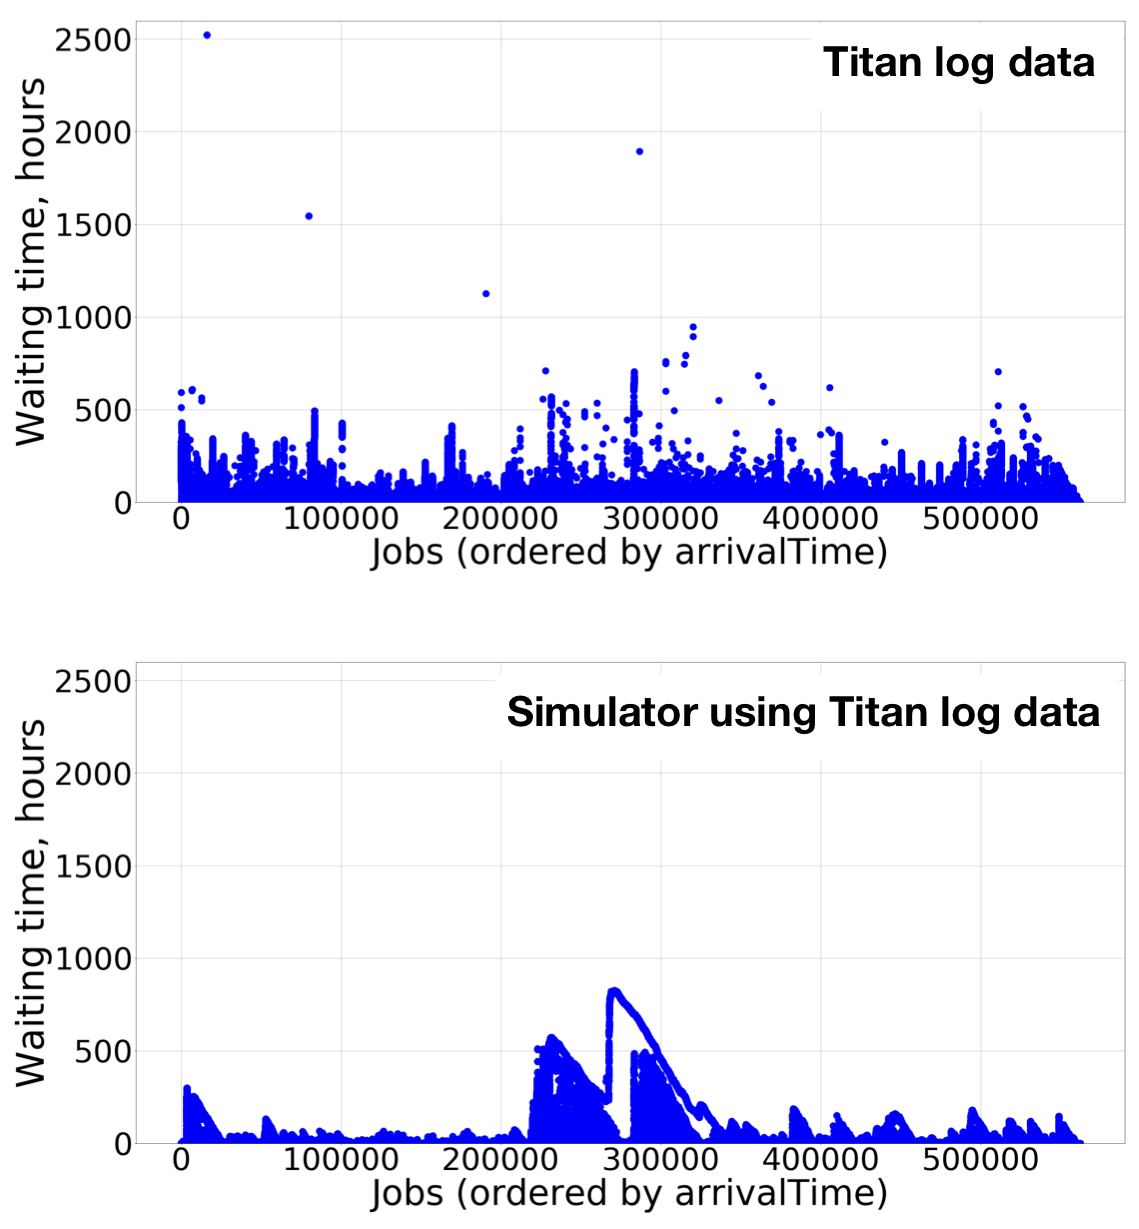
\includegraphics[width=0.45\textwidth]{pics/simulator-testing.png}
    \caption{Job waiting times based on Titan log data and Simulator log data with initial parameters from Titan log data (waiting time, hours - Titan: mean=6.21, std=29.77; Simulator: mean=30.51, std=97.34)}
    \label{fig-simulator-testing} 
\end{figure}

Figure~\ref{fig-simulator-load-1y} shows the load of the simulated nodes (i.e., the number of busy nodes at every simulated time unit, seconds) during the simulation process of jobs described earlier. The average utilization rate of the set of service nodes is 88.2 \%.

\begin{figure}
    \centering
    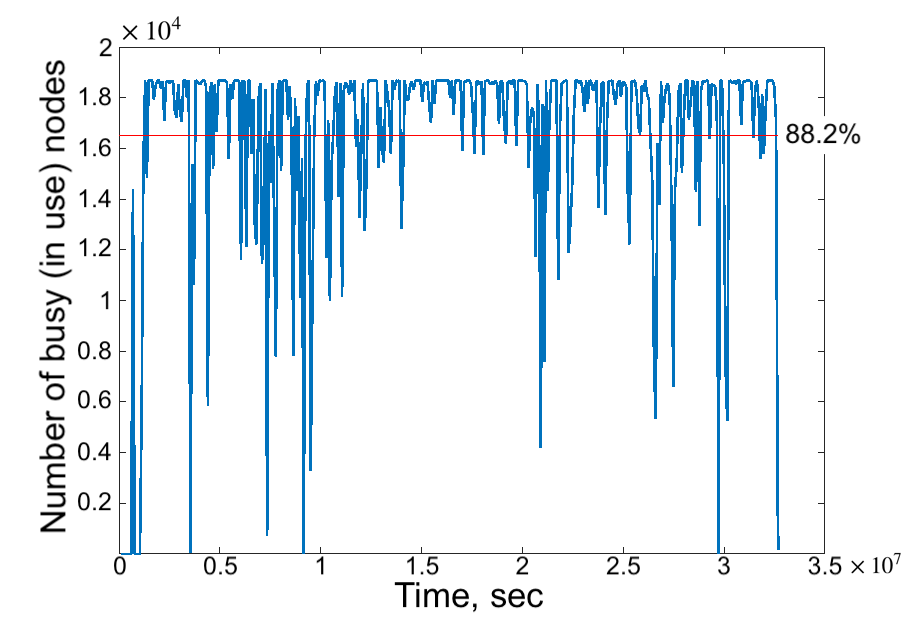
\includegraphics[width=0.45\textwidth]{pics/simulator-load-1y.png}
    \caption{The load of simulated service nodes (18,688 nodes)}
    \label{fig-simulator-load-1y} 
\end{figure}


\subsection{Analysis of Titan log data}
\label{sec-experiments-3}
Conducted experiments are based on obtained the Titan supercomputer log data that were used for the quantitative model. The following information was extracted from the log per job: i) arrival timestamp (time when the job was queued); ii) execution start timestamp (i.e., startTime); iii) completion timestamp (i.e., endTime); iv) the number of requested nodes (1 node = 16 cores in Titan); v) requested walltime.

As the first approach in analysis there were no separation of jobs from different projects, jobs were grouped only based on their sizes. Further analysis was applied on jobs from just one project to extend the potential applicability of our model.

\subsubsection{Analysis using log data of all projects} \label{sec-experiments-3-1}

The following analysis actions are applied:
\begin{itemize}
    \item all jobs are divided into categories according to the number of required nodes and the volume of walltime requested (every category corresponds to a particular Titan's bin, where \textit{bin} is a group of jobs that are treated equally);
    \item for each category the following values are calculated: the expected value and variance of random variables describing waiting time in the queue and the utilization achieved by a single job;
    \item obtained values were used as input data in equation for the quantitative model to calculate the probability that jobs of a given category will be able to utilize provided allocation in 3 months;
    \item job launching scheme: one stream and there is always one job in the queue.
\end{itemize}

The outcome of the performed analysis is presented by the set of 5 plots (one per Titan's bin) in Figure~\ref{fig-proj-all-probability-distr} (outperformed groups are highlighted at the legend). Log data was collected for the period from May 2017 to April 2018.

\begin{figure}
    \centering
    \begin{subfigure}{.5\textwidth}
        \centering
        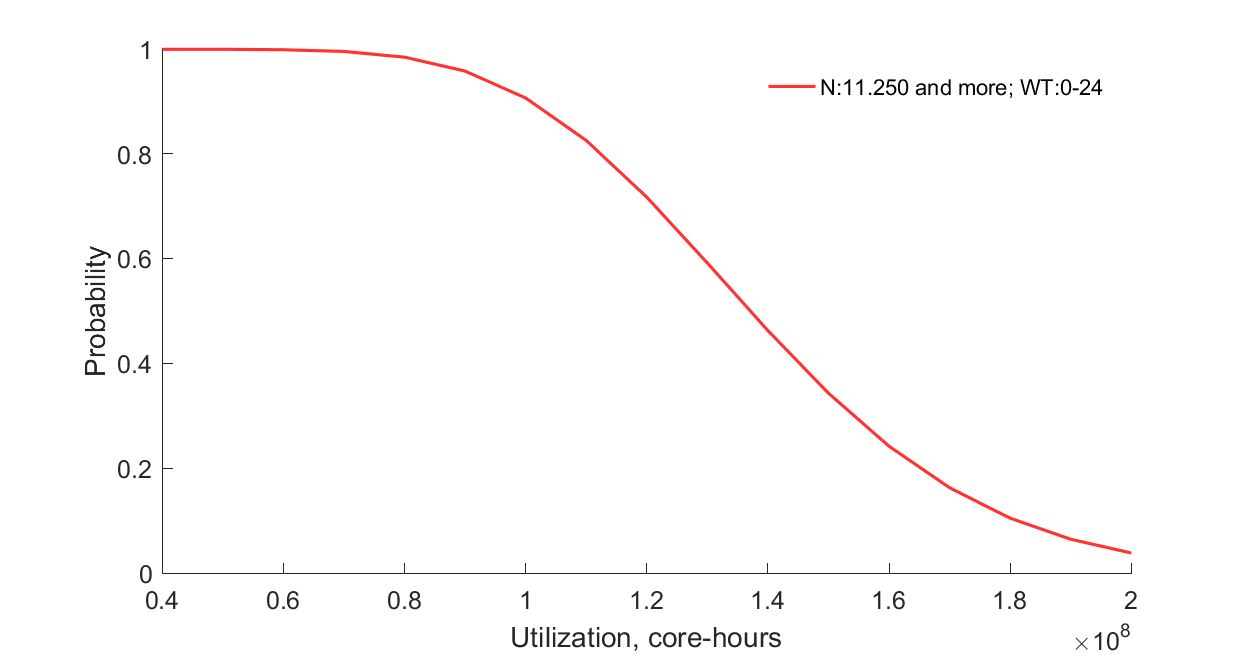
\includegraphics[width=.83\linewidth]{pics/proj-all-probability-distr-bin1.png}
        \caption{Bin-1 | nodes: [11,250:18,688]; walltime, h: [0:24]}
    \end{subfigure}
    \begin{subfigure}{.5\textwidth}
        \centering
        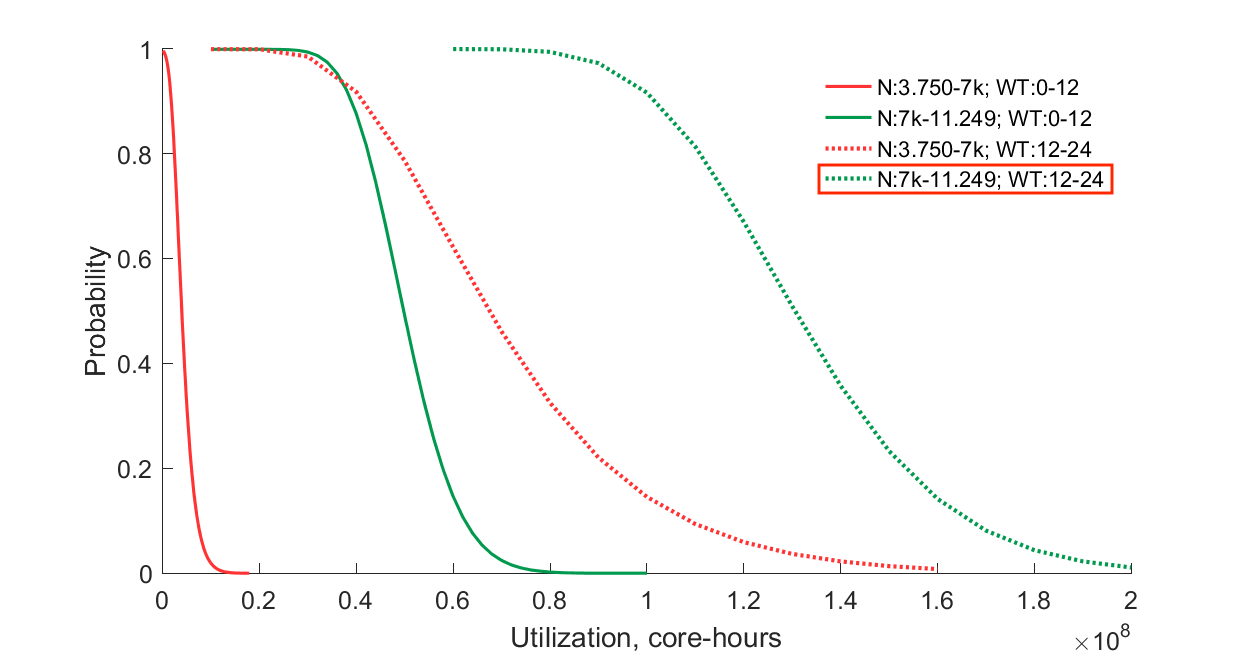
\includegraphics[width=.83\linewidth]{pics/proj-all-probability-distr-bin2.png}
        \caption{Bin-2 | nodes: [3,750:11,249]; walltime, h: [0:24]}
    \end{subfigure}
    \begin{subfigure}{.5\textwidth}
        \centering
        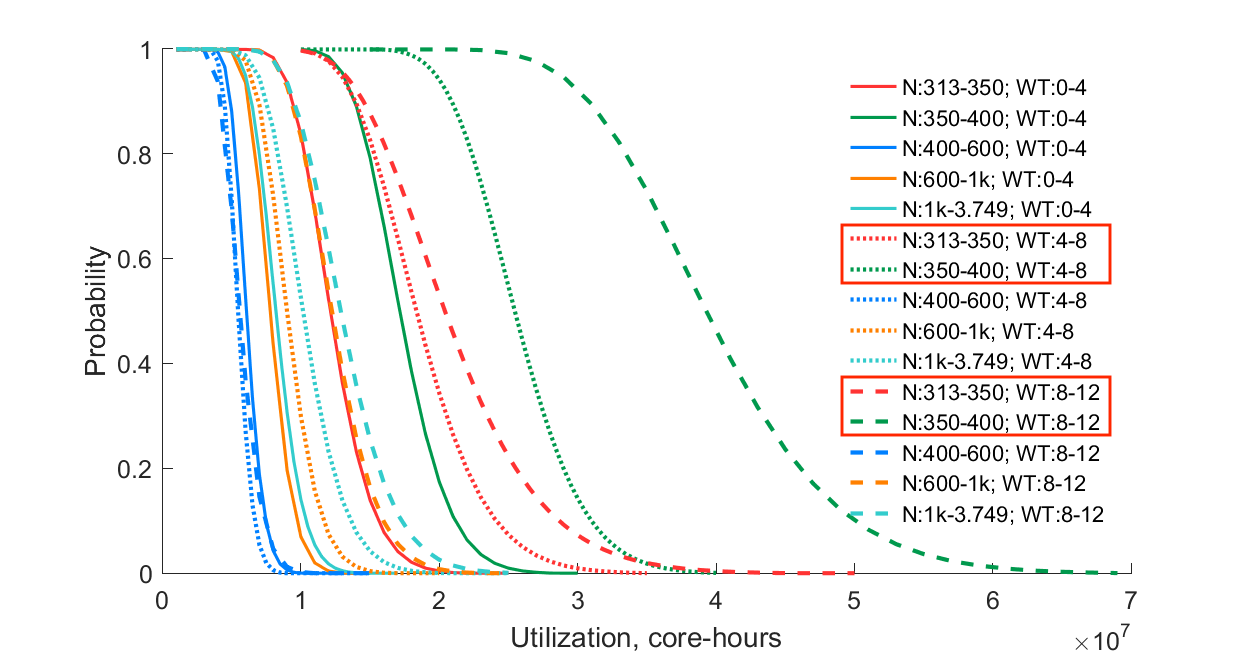
\includegraphics[width=.83\linewidth]{pics/proj-all-probability-distr-bin3.png}
        \caption{Bin-3 | nodes: [313:3,749]; walltime, h: [0:12]}
    \end{subfigure}
    \begin{subfigure}{.5\textwidth}
        \centering
        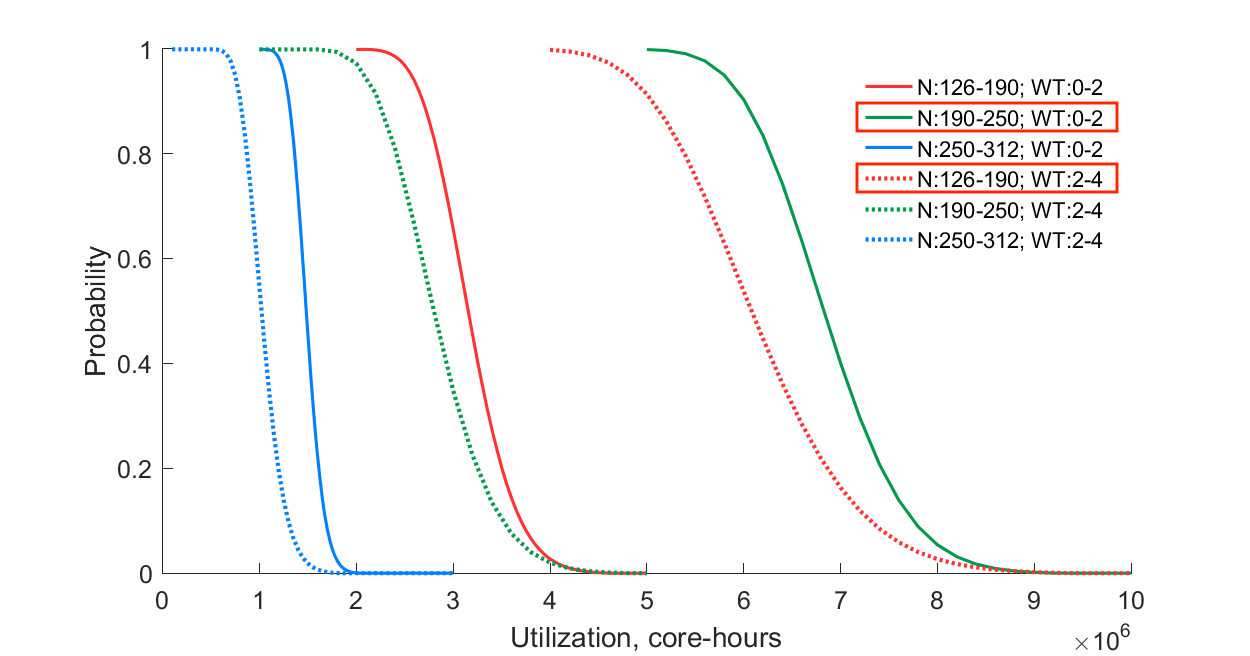
\includegraphics[width=.83\linewidth]{pics/proj-all-probability-distr-bin4.png}
        \caption{Bin-4 | nodes: [126:312]; walltime, h: [0:4]}
    \end{subfigure}
    \begin{subfigure}{.5\textwidth}
        \centering
        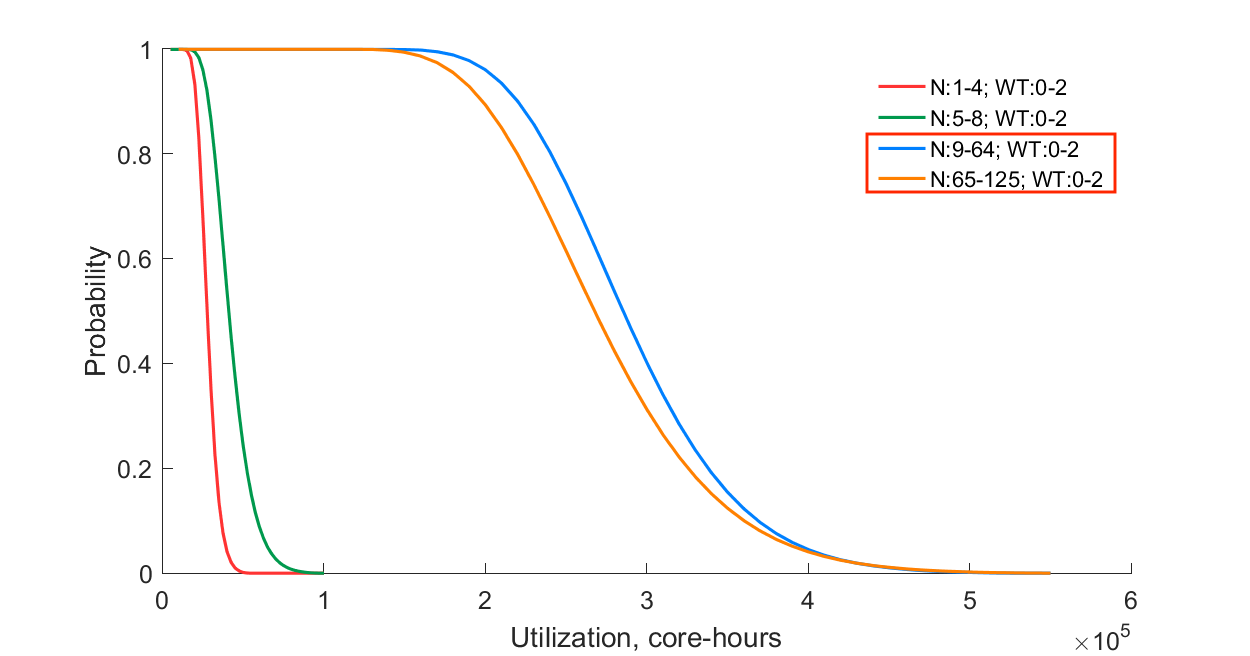
\includegraphics[width=.83\linewidth]{pics/proj-all-probability-distr-bin5.png}
        \caption{Bin-5 | nodes: [1:125]; walltime, h: [0:2]}
    \end{subfigure}
    \caption{Probability distributions of utilization of allocation time during 3 months per Titan's bins (based on Titan log data for 12 months)}
    \label{fig-proj-all-probability-distr}
\end{figure}

\subsubsection{Analysis using log data of one project (HEP110)} \label{sec-experiments-3-2}

Project HEP110 is associated with ALCC program, and computing jobs running under this project are from PanDA for the ATLAS experiment at LHC, CERN (actual ATLAS data wasn't in use for the current analysis, neither any data from PanDA). The outcome of the performed analysis for the project HEP110 is presented by the set of 2 plots (using jobs ``execution time'' and ``walltime''/``requested processing time'') in Figure~\ref{fig-hep110-probability-distr}.

\begin{figure}
    \centering
    \begin{subfigure}{.48\textwidth}
        \centering
        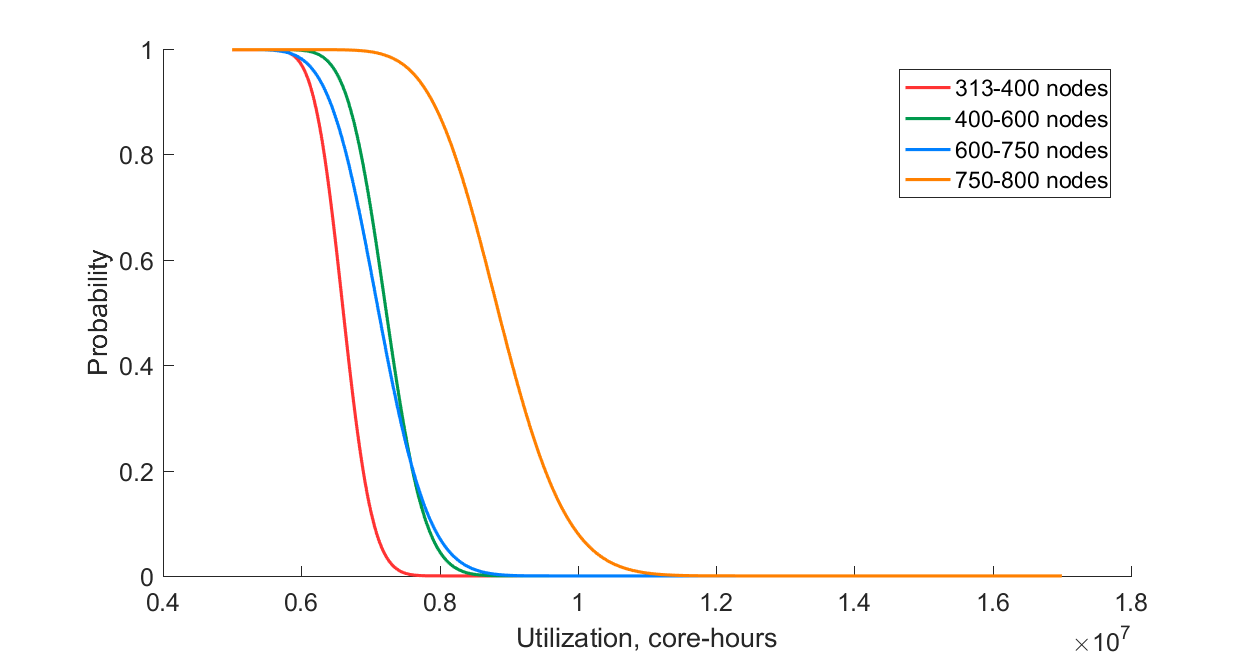
\includegraphics[width=.98\linewidth]{pics/hep110-probability-distr-exectime.png}
        \caption{Based on provided real execution time}
    \end{subfigure}
    \begin{subfigure}{.48\textwidth}
        \centering
        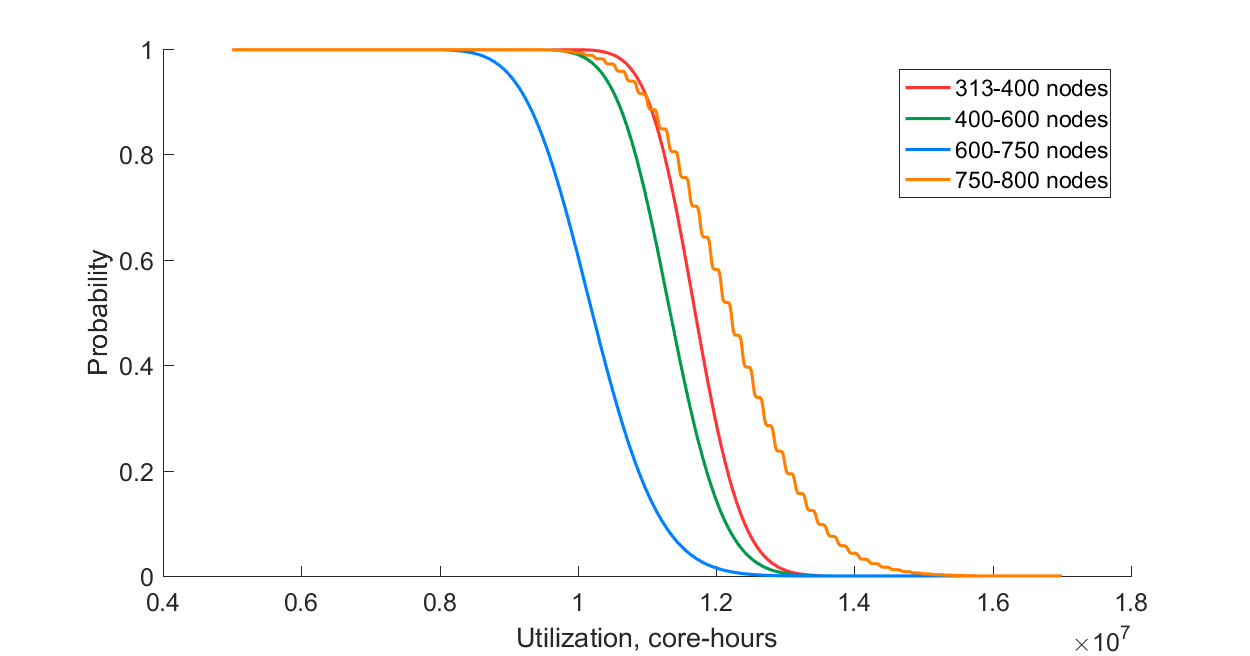
\includegraphics[width=.98\linewidth]{pics/hep110-probability-distr-walltime.png}
        \caption{Based on requested wall time}
    \end{subfigure}
    \caption{Probability distributions of utilization of allocation time during 3 months for HEP110 project at the Titan supercomputer (based on Titan log data for 6 months)}
    \label{fig-hep110-probability-distr}
\end{figure}



\section{Conclusion and discussion}
\label{sec-conclusions}
Developed tools provide possibility to adjust jobs parameters to regulate and improve the probability of utilizing a given allocation for a given project. Further work for the proposed approach improvement includes reinforcement of applied requirements (i.e., decrease the number of applied assumptions for the developed model and simulator). The model and simulator are preliminary and require further tuning, to understand the accuracy and sensitivity (to initial conditions, training duration, workload types). This early work will be extended to consider different kinds of workflows as well as different types of workloads of heterogeneous resources.



\begin{acknowledgements}
This research used resources of the Oak Ridge Leadership Computing Facility at the Oak Ridge National Laboratory, which is supported by the Office of Science of the U.S. Department of Energy under Contract No. DE-AC05-00OR22725. We also would like to express our appreciation to the Advanced Scientific Computing Research (ASCR) Leadership Computing Challenge (ALCC) and to all involved in this project, especially to OLCF working group. This work was funded in part by the Russian Ministry of Science and Education under contract No. 14.Z50.31.0024.
\end{acknowledgements}


% BibTeX users please use one of
%\bibliographystyle{spbasic}      % basic style, author-year citations
%\bibliographystyle{spmpsci}      % mathematics and physical sciences
%\bibliographystyle{spphys}       % APS-like style for physics
%\bibliography{}   % name your BibTeX data base

% Non-BibTeX users please use
\begin{thebibliography}{}
\bibitem{ref-qespera}
Murali, P., Vadhiyar, S.: Qespera: an adaptive framework for prediction of queue waiting times in supercomputer systems. Concurrency Computat.: Pract. Exper. \textbf{28}(9), 2685--2710 (2016) doi:10.1002/cpe.3735

\bibitem{ref-qbets}
Nurmi, D., Brevik, J., Wolski, R.: QBETS: Queue Bounds Estimation from Time Series. In: Frachtenberg, E., Schwiegelshohn, U. (eds.) Job Scheduling Strategies for Parallel Processing, Lecture Notes in Computer Science \textbf{4942}, pp.76--101. Springer, Berlin, Heidelberg (2008) doi:10.1007/978-3-540-78699-3\_5

\bibitem{ref-yang}
Yang, L.T., Ma, X., Mueller, F.: Cross-Platform Performance Prediction of Parallel Applications Using Partial Execution. In: Proceedings of the ACM/IEEE 2005 Supercomputing Conference, SC'05, pp.111--120 (2005) doi:10.1109/SC.2005.20

\bibitem{ref-guo}
Guo, J., Nomura, A., Barton, R., Zhang, H., Matsuoka, S.: Machine Learning Predictions for Underestimation of Job Runtime on HPC System. In: Yokota, R., Wu, W. (eds.) Supercomputing Frontiers, Lecture Notes in Computer Science, \textbf{10776}, pp.179--198. Springer, Cham (2018) doi:10.1007/978-3-319-69953-0\_11

\bibitem{ref-lerida}
Lérida, J.L., Solsona, F., Giné, F., Hanzich, M., García, J.R., Hernández, P.: MetaLoRaS: A Re-scheduling and Prediction MetaScheduler for Non-dedicated Multiclusters. In: Cappello, F., Herault, T., Dongarra, J. (eds.) Recent Advances in Parallel Virtual Machine and Message Passing Interface, Lecture Notes in Computer Science, \textbf{4757}, pp.195--203. Springer, Berlin, Heidelberg (2007) doi:10.1007/978-3-540-75416-9\_30

\bibitem{ref-sotiriadis}
Sotiriadis, S., Bessis, N., Antonopoulos, N.: Towards Inter-cloud Schedulers: A Survey of Meta-scheduling Approaches. In: 6th IEEE International Conference on P2P, Parallel, Grid, Cloud and Internet Computing, pp.59--66 (2011) doi:10.1109/3PGCIC.2011.19

\bibitem{ref-legrand}
Legrand, A., Trystram, D., Zrigui, S.: Adapting Batch Scheduling to Workload Characteristics: What can we expect From Online Learning? In: 33rd IEEE International Parallel \& Distributed Processing Symposium (IPDPS), pp.1--10 (2019)

\bibitem{ref-panda}
Barreiro Megino, F.H., De, K., Klimentov, A., Maeno, T., Nilsson, P., Oleynik, D., Padolski, S., Panitkin, S., Wenaus, T.: PanDA for ATLAS distributed computing in the next decade. J. Phys. Conf. Ser. \textbf{898}(5), 052002 (2017) doi:10.1088/1742-6596/898/5/052002

\bibitem{ref-atlas}
ATLAS Collaboration: The ATLAS Experiment at the CERN Large Hadron Collider. JINST \textbf{3}, S08003 (2008)

\bibitem{ref-titan-prodsys}
Barreiro Megino, F.H., De, K., Jha, S., Klimentov, A., Maeno, T., Nilsson, P., Oleynik, D., Padolski, S., Panitkin, S., Wells, J., Wenaus, T.: Integration of Titan supercomputer at OLCF with ATLAS Production System. J. Phys. Conf. Ser. \textbf{898}(9), 092002 (2017) doi:10.1088/1742-6596/898/9/092002

\bibitem{ref-saga}
Goodale, T., Jha, S., Kaiser, H., Kielmann, T., Kleijer, P., Von Laszewski, G., Lee, C.A., Merzky, A., Rajic, H.L., Shalf, J.: SAGA: A Simple API for Grid Applications. High-level application programming on the Grid. Comput. Methods Sci. Technol. \textbf{12}(1), 7--20 (2006) doi:10.12921/cmst.2006.12.01.07-20

\bibitem{ref-queueing-theory}
Cooper, R.B.: Introduction to Queueing Theory, 2nd Ed. Elsevier/North-Holland (1981)

\bibitem{ref-kendall}
Kendall, D.G.: Some Problems in the Theory of Queues. J. Royal Stat. Soc. Ser. B Methodol. \textbf{13}(2), 151--185 (1951)

\bibitem{ref-qss}
Titov, M., et al.: Queueing System Simulator (QSS) [software], \url{https://github.com/ATLAS-Titan/allocation-modeling} [accessed on 2020-02-10]


\end{thebibliography}

\clearpage
\appendix
\section{Derivation of the quantitative model} \label{appendix-model-derivation}

\textit{Given assumptions}:
\begin{enumerate}
    \item Project $Pr$;
    \item Jobs $J$ of project $Pr$;
    \item Jobs $J$ require $N$ nodes, where $N$ is a random variable with expected value $\mu_{N}$ and variance $\sigma_{N}^2$;
    \item Jobs $J$ require walltime $E$, where $E$ is a random variable with expected value $\mu_{E}$ and variance $\sigma_{E}^2$;
    \item Execution times of jobs $J$ equal to their walltime values;
    \item Jobs $J$ come into the supercomputer queue sequentially: next job is allocated to the queue after the previous one has left the queue to computing nodes;
    \item Duration of waiting time in the queue for jobs $J$ is described by a random variable $Q$ with expected value $\mu$ and variance $\sigma^2$.
\end{enumerate}
\textit{Values to find}:
$P(U > U_0)$ - the probability that utilization $U$ during the time interval $T_0$ will exceed the predefined value $U_0$, where $T_0$ is big.

\textit{Solution}.
Using the Law of total probability we can write the following equation:
\begin{equation}
    \label{eq-1}
    P(U > U_0) = \sum\limits_{n=1}^{\infty}P(U(n) > U_0) P(n)
\end{equation}
where $U(n)$ is a random variable for utilization achieved by $n$ sequential jobs $J$; $P(n)$ is a probability that during the time $T_0$ exactly $n$ jobs $J$ will be running. We assume that $T_0$ is big, so values of $P(n)$ for the first several $n$ (e.g., for $n$ from 1 to 99) are equal to zero, thus the sum would start with $n=100$.

To calculate $P(n)$ let's consider a random variable $T(n)$ describing the time required to run $n$ sequential jobs $J$. Taking into account one of the assumptions (6) we can write:
\begin{equation}
    \label{eq-2}
    T(n) = \sum\limits_{i=1}^{n}Q_{i}
\end{equation}
where $Q_{i} = Q$ is a random variable describing duration of waiting time in the queue for the job $J_{i}$. And, using Central limit theorem we can write for big values of $n$:
\begin{equation}
    \label{eq-3}
    \sum\limits_{i=1}^{n}Q_{i} \approx N(n\mu, n\sigma^2)
\end{equation}
where $N(\mu, \sigma^2)$ is a normal distribution with expected value $\mu$ and variance $\sigma^2$; $\mu$ is an expected value of a random variable $Q$ describing duration of waiting time in the queue for jobs $J$; $\sigma^2$ is a variance of a random variable $Q$ describing duration of waiting time in the queue for jobs $J$.

The probability $P(n)$ can be rewritten as following:
\begin{equation}
    \label{eq-4}
    P(n_0) = P(n \geq n_0) - P(n \geq n_0 + 1)
\end{equation}
where $P(n_0)$ is a probability that during the time $T_0$ precisely $n_0$ jobs $J$ will be running; $P(n \geq n_0)$ is a probability that during the time $T_0$ not less than $n_0$ jobs $J$ will be running. We can mention that the event $n \geq n_0$ (during the time $T_0$ not less than $n_0$ jobs $J$ will be running) is equal to the event $T(n_0) \leq T_0$ (the time required to run $n_0$ jobs $J$ is less than or equal to the time $T_0$). Considering that we have: $P(n \geq n_0) = P(T(n_0) \leq T_0)$ and $P(n \geq n_0 + 1) = P(T(n_0 + 1) \leq T_0)$. Thus, inserting these equations into Equation \ref{eq-4} and using Equations \ref{eq-2} and \ref{eq-3} we can have the following:
\begin{equation}
    \label{eq-5}
    \begin{multlined}
    P(n_0) = P(N(n_0\mu, n_0\sigma^2) \leq T_0) \  - \\
             \shoveleft[1cm]{P(N((n_0 + 1)\mu, (n_0 + 1)\sigma^2) \leq T_0)}
    \end{multlined} 
\end{equation}

This equation can be updated by using the probability density of the normal distribution:
\begin{equation}
    \label{eq-6}
    \begin{multlined}
    P(n_0) = \int_{-\infty}^{T_0}f(x, n_0\mu, n_0\sigma^2)dx \  - \\
             \shoveleft[1cm]{\int_{-\infty}^{T_0}f(x, (n_0 + 1)\mu, (n_0 + 1)\sigma^2)dx}
    \end{multlined}
\end{equation}
where $f(x, \mu, \sigma^2)$ is a function of probability density of the normal distribution $N(\mu, \sigma^2)$.

To calculate value of $P(U(n) > U_0)$ in Equation \ref{eq-1} let's write a random variable $U(n)$ as a sum of random variables $U_{i}$ describing utilization of the single job $J_{i}$: $U(n_0) = \sum_{i=1}^{n_0}U_{i}$. Assuming that all random variables $U_{i}$ have the same expected values (let's denote them as $\mu_{U}$) and variances (let's denote them as $\sigma_{U}^2$) and using as before the Central limit theorem we can write for big values of $n$:
\begin{equation}
    \label{eq-7}
    U(n_0) = \sum_{i=1}^{n_0}U_{i} \approx N(n_0\mu_{U}, n_0\sigma_{U}^2)
\end{equation}

Using the probability density of the normal distribution and Equation \ref{eq-7} we can write $P(U(n) > U_0)$ in a way:
\begin{equation}
    \label{eq-8}
    P(U(n) > U_0) = \int_{U_0}^{\infty}f(x, n\mu_{U}, n\sigma_{U}^2)dx
\end{equation}

To get the final equation we insert Equations \ref{eq-6} and \ref{eq-8} into the Equation \ref{eq-1}:
\begin{equation}
    \label{eq-9}
    \begin{multlined}
    P(U > U_0) = \sum\limits_{n=100}^{\infty} 
                 \bigg[ \int_{U_0}^{\infty}f(x, n\mu_{U}, n\sigma_{U}^2)dx \  \times \\
                 \bigg( \int_{-\infty}^{T_0}f(x, n\mu, n\sigma^2)dx \  - \\
                 \int_{-\infty}^{T_0}f(x, (n+1)\mu, (n+1)\sigma^2)dx \bigg) \bigg]
    \end{multlined}
\end{equation}

The outcome of the Equation~\ref{eq-9} is the probability that the utilization of resources, which is achieved by a sequential set of processed jobs using capabilities of the supercomputer during the time interval $T_0$, is greater than the predefined value $U_0$. It implies that:
\begin{itemize}
	\item Utilization of every single job is described by a random variable with the expected value $\mu_{U}$ and the variance $\sigma_{U}^2$;
	\item The time interval between launches of sequential jobs is described by a random variable with the expected value $\mu$ and the variance $\sigma^2$.
\end{itemize}

Generally, the distribution of a random variable that describes the size of the job in a way as the number of occupied cores (denote this random variable as $N$) and the distribution of a random variable that describes the time to complete for a single job (denote this random variable as $E$) are more commonly known compare to the distribution of a random variable that describes the utilization achieved by a single job (denote this random variable as $U$). Since, the utilization of a single job is a product of the amount of the used resources by the time to complete this job, then, in case of mutual independence of random variables $N$ and $E$, the values $\mu_U$ and $\sigma_{U}^2$ can be found by the following equations:
\begin{equation}
    \label{eq-10}
    \mu_U = \mu_N \mu_E \\
\end{equation}
where $\mu_N$ is the expected value of the random variable $N$; $\mu_E$ is the expected value of the random variable $E$.
\begin{equation}
    \label{eq-11}
    \sigma_{U}^2 = \sigma_{N}^2 \sigma_{E}^2 + \mu_N \sigma_{E}^2 + \mu_E \sigma_{N}^2
\end{equation}
where $\sigma_{N}^2$ is the variance of the random variable $N$; $\sigma_{E}^2$ is the variance of the random variable E.


\end{document}
